\documentclass[a4paper,11pt,twoside]{ThesisStyle}

\usepackage{lmodern}
\usepackage{subfig}
\usepackage{enumitem}
\usepackage{url}
\usepackage{algorithm}
\usepackage{array}
\usepackage[pdftex]{adjustbox}

%\makeatletter
%\setlength{\@fptop}{0pt}
%\makeatother
\usepackage{amsmath,amssymb}             % AMS Math
% \usepackage[french]{babel}
\usepackage[latin1]{inputenc}
\usepackage[T1]{fontenc}
\usepackage[left=1.2in,right=1.2in,top=0.8in,bottom=1.1in,includefoot,includehead,headheight=13.6pt]{geometry}
\renewcommand{\baselinestretch}{1.05}

% Table of contents for each chapter

\usepackage[nottoc, notlof, notlot]{tocbibind}
\usepackage{minitoc}
\setcounter{minitocdepth}{2}
\mtcindent=15pt
% Use \minitoc where to put a table of contents

\usepackage{aecompl}

% Glossary / list of abbreviations

\usepackage[intoc]{nomencl}
\renewcommand{\nomname}{List of Abbreviations}

\makenomenclature

% My pdf code

\usepackage{ifpdf}

\ifpdf
  \usepackage[pdftex]{graphicx}
  \DeclareGraphicsExtensions{.jpg}
  \usepackage[a4paper,pagebackref,hyperindex=true]{hyperref}
\else
  \usepackage{graphicx}
  \DeclareGraphicsExtensions{.ps,.eps}
  \usepackage[a4paper,dvipdfm,pagebackref,hyperindex=true]{hyperref}
\fi

\graphicspath{{.}{images/}}

% nicer backref links
\renewcommand*{\backref}[1]{}
\renewcommand*{\backrefalt}[4]{%
\ifcase #1 %
(Not cited.)%
\or
(Cited on page~#2.)%
\else
(Cited on pages~#2.)%
\fi}
\renewcommand*{\backrefsep}{, }
\renewcommand*{\backreftwosep}{ and~}
\renewcommand*{\backreflastsep}{ and~}

% Links in pdf
\usepackage{color}
\definecolor{linkcol}{rgb}{0,0,0.4} 
\definecolor{citecol}{rgb}{0.5,0,0} 

% Change this to change the informations included in the pdf file

% See hyperref documentation for information on those parameters

\hypersetup
{
bookmarksopen=true,
pdftitle="...",
pdfauthor="...", 
pdfsubject="...", %subject of the document
%pdftoolbar=false, % toolbar hidden
pdfmenubar=true, %menubar shown
pdfhighlight=/O, %effect of clicking on a link
colorlinks=true, %couleurs sur les liens hypertextes
pdfpagemode=None, %aucun mode de page
pdfpagelayout=SinglePage, %ouverture en simple page
pdffitwindow=true, %pages ouvertes entierement dans toute la fenetre
linkcolor=linkcol, %couleur des liens hypertextes internes
citecolor=citecol, %couleur des liens pour les citations
urlcolor=linkcol %couleur des liens pour les url
}

% definitions.
% -------------------

\setcounter{secnumdepth}{3}
\setcounter{tocdepth}{2}

% Some useful commands and shortcut for maths:  partial derivative and stuff

\newcommand{\pd}[2]{\frac{\partial #1}{\partial #2}}
\def\abs{\operatorname{abs}}
\def\argmax{\operatornamewithlimits{arg\,max}}
\def\argmin{\operatornamewithlimits{arg\,min}}
\def\diag{\operatorname{Diag}}
\newcommand{\eqRef}[1]{(\ref{#1})}

\usepackage{rotating}                    % Sideways of figures & tables
%\usepackage{bibunits}
%\usepackage[sectionbib]{chapterbib}          % Cross-reference package (Natural BiB)
%\usepackage{natbib}                  % Put References at the end of each chapter
                                         % Do not put 'sectionbib' option here.
                                         % Sectionbib option in 'natbib' will do.
\usepackage{fancyhdr}                    % Fancy Header and Footer

% \usepackage{txfonts}                     % Public Times New Roman text & math font
  
%%% Fancy Header %%%%%%%%%%%%%%%%%%%%%%%%%%%%%%%%%%%%%%%%%%%%%%%%%%%%%%%%%%%%%%%%%%
% Fancy Header Style Options

\pagestyle{fancy}                       % Sets fancy header and footer
\fancyfoot{}                            % Delete current footer settings

%\renewcommand{\chaptermark}[1]{         % Lower Case Chapter marker style
%  \markboth{\chaptername\ \thechapter.\ #1}}{}} %

%\renewcommand{\sectionmark}[1]{         % Lower case Section marker style
%  \markright{\thesection.\ #1}}         %

\fancyhead[LE,RO]{\bfseries\thepage}    % Page number (boldface) in left on even
% pages and right on odd pages
\fancyhead[RE]{\bfseries\nouppercase{\leftmark}}      % Chapter in the right on even pages
\fancyhead[LO]{\bfseries\nouppercase{\rightmark}}     % Section in the left on odd pages

\let\headruleORIG\headrule
\renewcommand{\headrule}{\color{black} \headruleORIG}
\renewcommand{\headrulewidth}{1.0pt}
\usepackage{colortbl}
\arrayrulecolor{black}

\fancypagestyle{plain}{
  \fancyhead{}
  \fancyfoot{}
  \renewcommand{\headrulewidth}{0pt}
}

\usepackage{algorithm}
\usepackage[noend]{algorithmic}

%%% Clear Header %%%%%%%%%%%%%%%%%%%%%%%%%%%%%%%%%%%%%%%%%%%%%%%%%%%%%%%%%%%%%%%%%%
% Clear Header Style on the Last Empty Odd pages
\makeatletter

\def\cleardoublepage{\clearpage\if@twoside \ifodd\c@page\else%
  \hbox{}%
  \thispagestyle{empty}%              % Empty header styles
  \newpage%
  \if@twocolumn\hbox{}\newpage\fi\fi\fi}

\makeatother
 
%%%%%%%%%%%%%%%%%%%%%%%%%%%%%%%%%%%%%%%%%%%%%%%%%%%%%%%%%%%%%%%%%%%%%%%%%%%%%%% 
% Prints your review date and 'Draft Version' (From Josullvn, CS, CMU)
\newcommand{\reviewtimetoday}[2]{\special{!userdict begin
    /bop-hook{gsave 20 710 translate 45 rotate 0.8 setgray
      /Times-Roman findfont 12 scalefont setfont 0 0   moveto (#1) show
      0 -12 moveto (#2) show grestore}def end}}
% You can turn on or off this option.
% \reviewtimetoday{\today}{Draft Version}
%%%%%%%%%%%%%%%%%%%%%%%%%%%%%%%%%%%%%%%%%%%%%%%%%%%%%%%%%%%%%%%%%%%%%%%%%%%%%%% 

\newenvironment{maxime}[1]
{
\vspace*{0cm}
\hfill
\begin{minipage}{0.5\textwidth}%
%\rule[0.5ex]{\textwidth}{0.1mm}\\%
\hrulefill $\:$ {\bf #1}\\
%\vspace*{-0.25cm}
\it 
}%
{%

\hrulefill
\vspace*{0.5cm}%
\end{minipage}
}

\let\minitocORIG\minitoc
\renewcommand{\minitoc}{\minitocORIG \vspace{1.5em}}

\usepackage{multirow}
\usepackage{slashbox}

\newenvironment{bulletList}%
{ \begin{list}%
	{$\bullet$}%
	{\setlength{\labelwidth}{25pt}%
	 \setlength{\leftmargin}{30pt}%
	 \setlength{\itemsep}{\parsep}}}%
{ \end{list} }

\newtheorem{definition}{D�finition}
\renewcommand{\epsilon}{\varepsilon}

% centered page environment

\newenvironment{vcenterpage}
{\newpage\vspace*{\fill}\thispagestyle{empty}\renewcommand{\headrulewidth}{0pt}}
{\vspace*{\fill}}



\begin{document}
%----------------------------------------------------------------------------------------
%	TITLE PAGE
%----------------------------------------------------------------------------------------
\let\cleardoublepage\clearpage 
\begin{titlepage}
\begin{figure}
\vspace{-2cm}
   \begin{minipage}[r]{0.46\linewidth}
   \hspace*{-1cm}
      
\includegraphics[scale=1.5,  width=.7\textwidth]{logocs.jpeg}
   \end{minipage} 
   \begin{minipage}[l]{0.46\linewidth}
   \hspace*{3.7cm}
      
\includegraphics[scale=1, width=.5\textwidth]{it4bi_logo.jpg}
   \end{minipage}
\end{figure}

\vspace*{0cm}
\begin{center}
\noindent \Huge \textbf{Decision Support and Business Intelligence} \\
\vspace*{0.4cm}
\noindent \Large \textit{\textbf{ Information Technologies for Business Intelligence}}\\
\vspace*{0.4cm}
\noindent \Huge \textbf{Master Thesis} \\

\vspace*{0.5cm}
\noindent \LARGE Oky  \textsc{Purwantiningsih} \\
\vspace*{0.5cm}
\begin{tabular}{c}
\hline\\
\noindent {\Huge \textbf{Visual Analytics }} \\
\noindent {\Huge \textbf{on Human Body Movement Data}} \\
\noindent {\Huge \textbf{Applied on Healthcare}} \\
\\
\hline\\
\end{tabular}
\vspace*{0.2cm}
\\
\noindent {\Large prepared at LIRMM and Universit\'{e} Paul Val\'{e}ry Montpellier} \\
\vspace*{0.2cm}
\noindent \large Submitted on September 10, 2015 \\
\vspace*{0.5cm}
\end{center}
\begin{center}
\noindent \large 
\begin{adjustbox}{width=1.2\textwidth,center}
\begin{tabular}{llcll}
      \textit{Advisor :}	& Arnaud \textsc{Sallaberry}		& - & LIRMM& arnaud.sallaberry@lirmm.fr\\
      & Jer\^{o}m\'{e} \textsc{Az\'{e}}		& - & LIRMM& jerome.aze@lirmm.fr\\
      \textit{Supervisor :}	& Nac\'{e}ra \textsc{Bennacer}		& - & Centrale Sup\'{e}lec& nacera.bennacer@supelec.fr\\
       \textit{In collaboration with :}	& S\'{e}bastien \textsc{Andary}		& - & NaturalPad & sebastien@naturalpad.fr\\
\end{tabular}
\end{adjustbox}
\end{center}
\begin{figure}[b]
   \vspace*{-2cm}
	\makebox[\linewidth]{
   \begin{minipage}[r]{0.46\linewidth}
   \hspace*{-1cm}
      
\includegraphics[scale=0.5,  width=.7\textwidth]{Logo_univ_paul_valery.jpg}
   \end{minipage} 
   \begin{minipage}[l]{0.46\linewidth}
   \hspace*{3.2cm}
      
\includegraphics[scale=0.5, width=.7\textwidth]{lirmm_logo2.jpg}
   \end{minipage}
   }

\end{figure}
\end{titlepage}
\sloppy

\titlepage


%----------------------------------------------------------------------------------------
%	ABSTRACT
%----------------------------------------------------------------------------------------

\begin{vcenterpage}
\noindent\rule[2pt]{\textwidth}{0.5pt}

\noindent{\large\textbf{Abstract:}}
Serious game is used in healthcare to perform patients' rehabilitation and training. An example of such game is Hammer and Planks which is used to rehabilitate patient with balance disorders. Utilizing motion sensing input devices (Kinect, Wii Balance Board), the game is played by moving player's body. However, it is difficult to assess the rehabilitation progress from the game. In this Master thesis we design and develop visualization interface to help healthcare professional make correct diagnostic of patients' progress and therefore enable them to set the difficulty level for future rehabilitation session.
\\
To achieve this objective, we developed a visualization application which enables healthcare professional to analyse gameplay from two different views: (i) Session Visualization which allows analysis on one session. With this view, users are able to identify the frequency of movement related to objects on the game (ii) Summary Visualization which allows movement analysis over several sessions. This view enables users to navigate and explore the evolution of movement throughout all of the sessions. Here we propose a clustering method based on hierarchical clustering to group similar movement pattern over sections of game horizontal x-axis. This view also enables users to analyse in which area of x-axis the movement frequently happened. The proposed visualization is illustrated with two case studies which demonstrate the ability of the application to assess the rehabilitation progress.
\\
{\large\textbf{Keywords:}}
Information Visualization, Visual Analytic, Movement Analysis, Hierarchical Clustering
\\
\noindent\rule[2pt]{\textwidth}{0.5pt}
\end{vcenterpage}

\dominitoc

\pagenumbering{roman}
\cleardoublepage
%----------------------------------------------------------------------------------------
%	ACKNOWLEDGMENTS
%----------------------------------------------------------------------------------------

\section*{Acknowledgments}

In the name of Allah, the Most Gracious and the Most Merciful.

Alhamdulillah, all praises to Allah for the strengths and His blessings in completing this thesis.

Firstly, I would like to express my sincere gratitude to my advisors Arnaud Sallaberry and Jer\^{o}m\'{e} Az\'{e} for their valuable guidance, detailed feedbacks, and continuous support. Without their help, I wouldn't be able to finish the research and complete the writing of this master thesis. Especially for Arnaud Salaberry, his patience and attention has made the development of the visualization application possible. I would also like to thank my supervisor  Nac\'{e}ra Bennacer for her insightful comments and feedbacks.

I am also thankful to S\'{e}bastien Andary of NaturalPad for his help regarding the Hammer and Planks game as well as providing the game application and data for the research. His valuable support has made the completion of this research possible.

My sincere thanks also goes to the Advanse Team in LIRMM, who gave me the opportunity to join their team as an intern and who provided access to their research facilities. Most importantly, for their understanding and support when I had medical difficulties during my internship.
My immense gratitude towards my colleague for their time and participation in providing the gameplay data set.


My gratitude goes to the IT4BI Consortium for giving me the opportunity and making all of this possible. 

I thank my friends for their company, support and motivation during the past six months. Thank you for the friendship and memories. I would also like to thank my parents for their continuous support and prayers.  

%----------------------------------------------------------------------------------------
%	TABLE OF CONTENTS, LIST OF FIGURES, LIST OF TABLES
%----------------------------------------------------------------------------------------

\tableofcontents
\newpage
\listoffigures
\newpage
\listoftables

\mainmatter
%----------------------------------------------------------------------------------------
%	CHAPTER
%----------------------------------------------------------------------------------------

\chapter{Introduction}
\label{chap:intro}

The advancement of gaming device technology such as Kinect, Wii Balance Board, Wii Remote, PlayStation Move, etc. has enabled players to control and interact with the game console through body movement. In healthcare, such technology are used in serious game which can help the users (doctors, patients, researchers, etc.)  perform health related activity such as patients' rehabilitation and training\cite{rahman,brezinka,green}. One example of such game is Hammer and Planks which was designed to train the equilibrium of patient with balance disorders (specifically for hemiplegic people)\cite{diloreto}. A person with hemiplegic is paralized on one side of the body\footnote{\url{http://www.hemihelp.org.uk/hemiplegia/what_is_hemiplegia}}. Therefore, the gameplay is designed so that the player has to move their body to right, left, front and back in order to train their affected side of the body. To support the purpose of rehabilitation, the healthcare professionals need to analyse the movement to  make a correct diagnostic of patients' progress and to adjust the difficulty level for the next rehabilitation session. In this thesis, I discuss the design of an interface to help healthcare professional to understand the data generated from the game.

\section{Motivation}

Hammer and Planks is a vertical shooter game. The game world is in a 2D environment vertically scrolling from top to bottom in which a player navigate a ship from left to right through moving his body(figure \ref{game_screenshot}). It tells the story of a pirate named John K. One day a meteor fell down on John's ship and ruin it. There is a little left from his boat but it is still enough to build a new basic boat with what's left. While navigating his ship to collect driftwood/plank to upgrade it (hence the name Hammer and Planks), he also wants to find the ship which showered meteor and destroyed his ship. Therefore, in the game a player has to defeat all enemies which come on his way and he has to avoid being destroyed by bullets, reefs and other obstacles. Throughout the game the player has to collect bonuses (planks) to improve the ship. The game is usually played in short and intense phase and thus requires a lot of concentration\cite{diloreto}.

Currently, the game provides some charts which visualize player's body movement with respect to the horizontal axis and vertical axis. However, the information that can be gathered from the visualization is not enough for the healthcare professional to be able to establish an informed diagnostic. It's hard to know how often the player move to right or left. It's also not possible to know to which type of events (ie. avoiding an enemy, catching the bonuses) the movement is related to. Which is crucial since the therapist need to know if the player is able to develop strategy to play the game overtime. The existing visualization also provides chart to show the evolution of player's performance and total movement for all game sessions. However, the evolution of player's body movement (horizontally or vertically) is not depicted.

The purpose of this thesis is to address the problem mentioned by proposing three types of visualization:(i)a visualization which provides information related to a certain type of event in the game and body movement for each one game session (ii)a visualization which represents a certain type of event, body movement, and the speed in which the event is occurring in one game session, and (iii)a visualization where healthcare professionals can analyze the evolution of player's body movement throughout all sessions. For the third visualization, there are two options in which the user can analyze the movement: by area of movement or by the number of movement in an area.

\begin{figure}
\centering
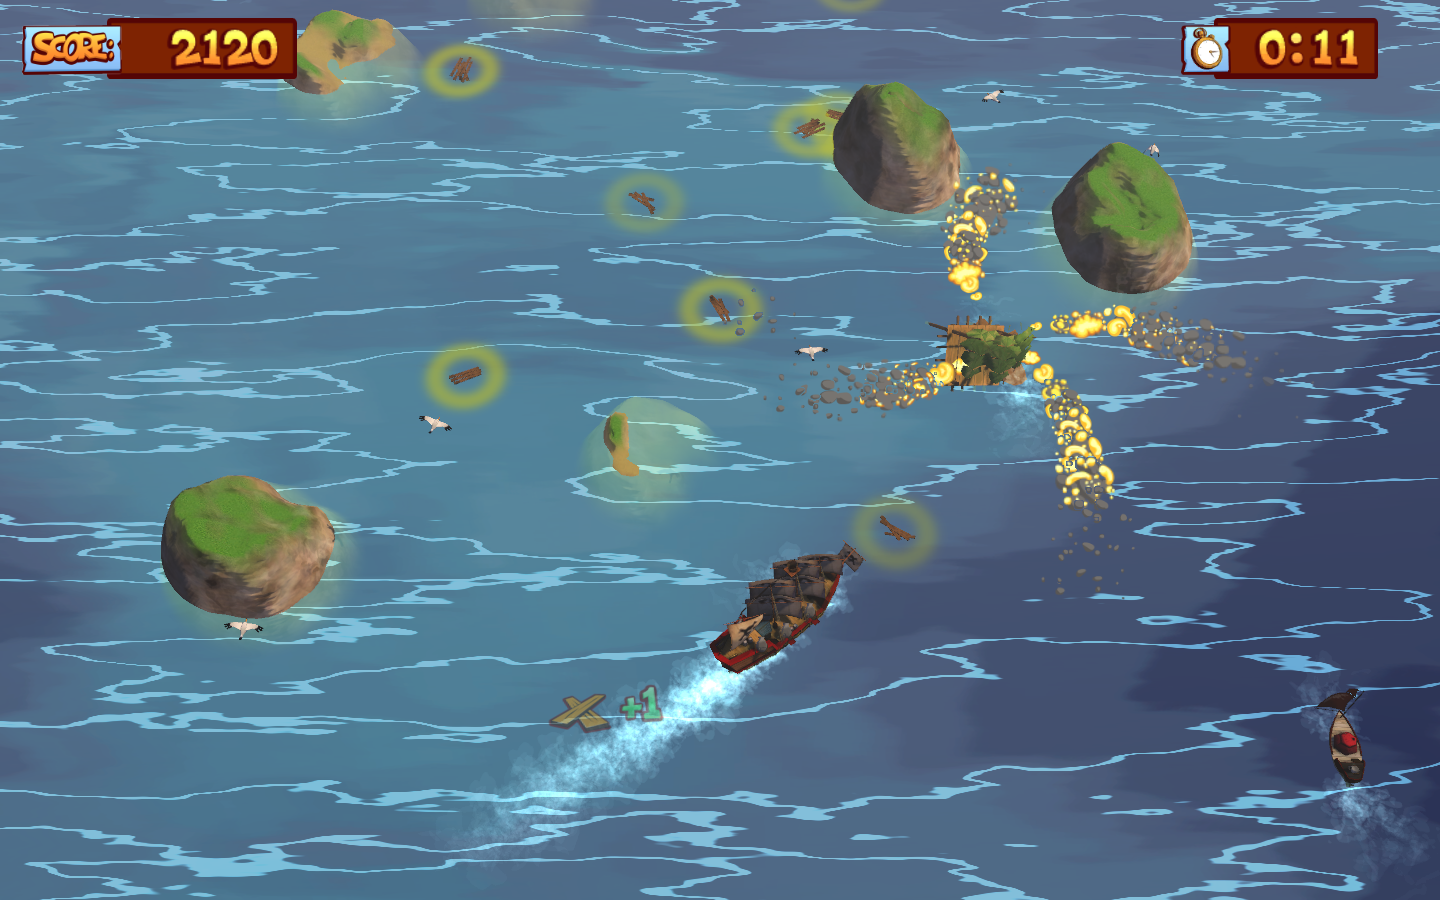
\includegraphics[width=110mm]{hp_game.png}
\caption{Hammer and Planks Screenshot \label{game_screenshot}}
\end{figure}


\section{Methodology}

To ensure that the visualization to be designed would satisfy the information needed by healthcare professionals, I followed the Nested Process Model proposed by Tamara Munzner \cite{Munzner:2009:NMV:1638611.1639181}. The model is divided into 4 levels: Domain Problem Characterization, Data/Operation Abstraction Design, Encoding/Interaction Technique Design, and Algorithm Design. These levels are nested; the output of a higher level will be the input for the lower level as shown in figure \ref{munzner_model}.

\begin{figure}
\centering
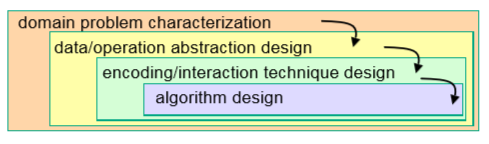
\includegraphics[width=100mm]{munzner_model.png}
\caption{Munzner's Visualization Design Model with four nested layers \label{munzner_model}}
\end{figure}

In domain problem characterization level, I discuss what kind of information needed by health professional from the visualization. The output of this level would be a list of tasks that need to be solved by the visualization application. I then identifies the data structure which can support these tasks in the Data/Operation Abstraction Design level. In the third level, a good visualization and interaction technique which can support the tasks will be defined. For this thesis, I leave out the algorithm design level since there is no new algorithm proposed.

\section{Thesis Outline}

The remainder of this thesis is organized as follows. Chapter 2 discuss the domain problem characterization. Chapter 3 explores related work. The data abstraction is presented in Chapter 4. The Visual Mapping and Interactive Functionality of the proposed visualization are discussed in details in Chapter 5. Chapter 6 provides some case studies used to evaluate the approach and finally, chapter 7 concludes the thesis.

\chapter{Domain Problem Characterization}
\label{chap:problem}

In order to clearly understand the problems faced by the healthcare professional in interpreting the gameplay into a meaningful therapy routine, first it is important to have an understanding of how the game is played. Based on this understanding, then it will be possible to find out what kind of information needed by defining questions usually asked by the users. In the end, visualization requirement elicitation will be done by translating each question into list of tasks. This chapter discusses each one of these steps in details.

\section{Hammer and Planks Game Dynamics}

Played with Kinect, it is possible to play Hammer and Planks in three different ways:
\begin{enumerate}
  \item BodyTilt:
  Player puts both arm in his/her hips and move the the upper body (from the waist up) to the right, left, forward or backward to navigate the boat(figure \ref{fig:movement_type} (left)). 
  \item HandPoint:
  Player lifts one of his/her forearm in front of the body with the palm facing forward. Navigating the boat can be done by moving the forearm to the right, left, forward, or backward(figure \ref{fig:movement_type} (right)).
  \item ShoulderCGE:
  Player lifts one of his/her arm in front of the body and bend the elbow. Moving the elbow up and down will navigate the boat up and down the screen.
\end{enumerate}

For both the BodyTilt and HandPoint there are three direction available: (i) Horizontal: the screen scrolls from top to bottom and player navigates the ship from left to right (ii) Vertical: the screen scrolls from right to left and player navigates the ship from top to bottom of the screen(iii) Both: the screen scrolls from top to bottom and player navigates the ship from left to right. He/she can also move the boat faster or slower by bending the upper body (BodyTilt) or arm (HandPoint) forward or backward . For ShoulderCGE there is only vertical direction. In this thesis, I only interested in games played using BodyTilt and HandPoint movement for both direction since the information generated are richer, thus harder for the specialist to understand.

%\begin{figure}
%\centering
%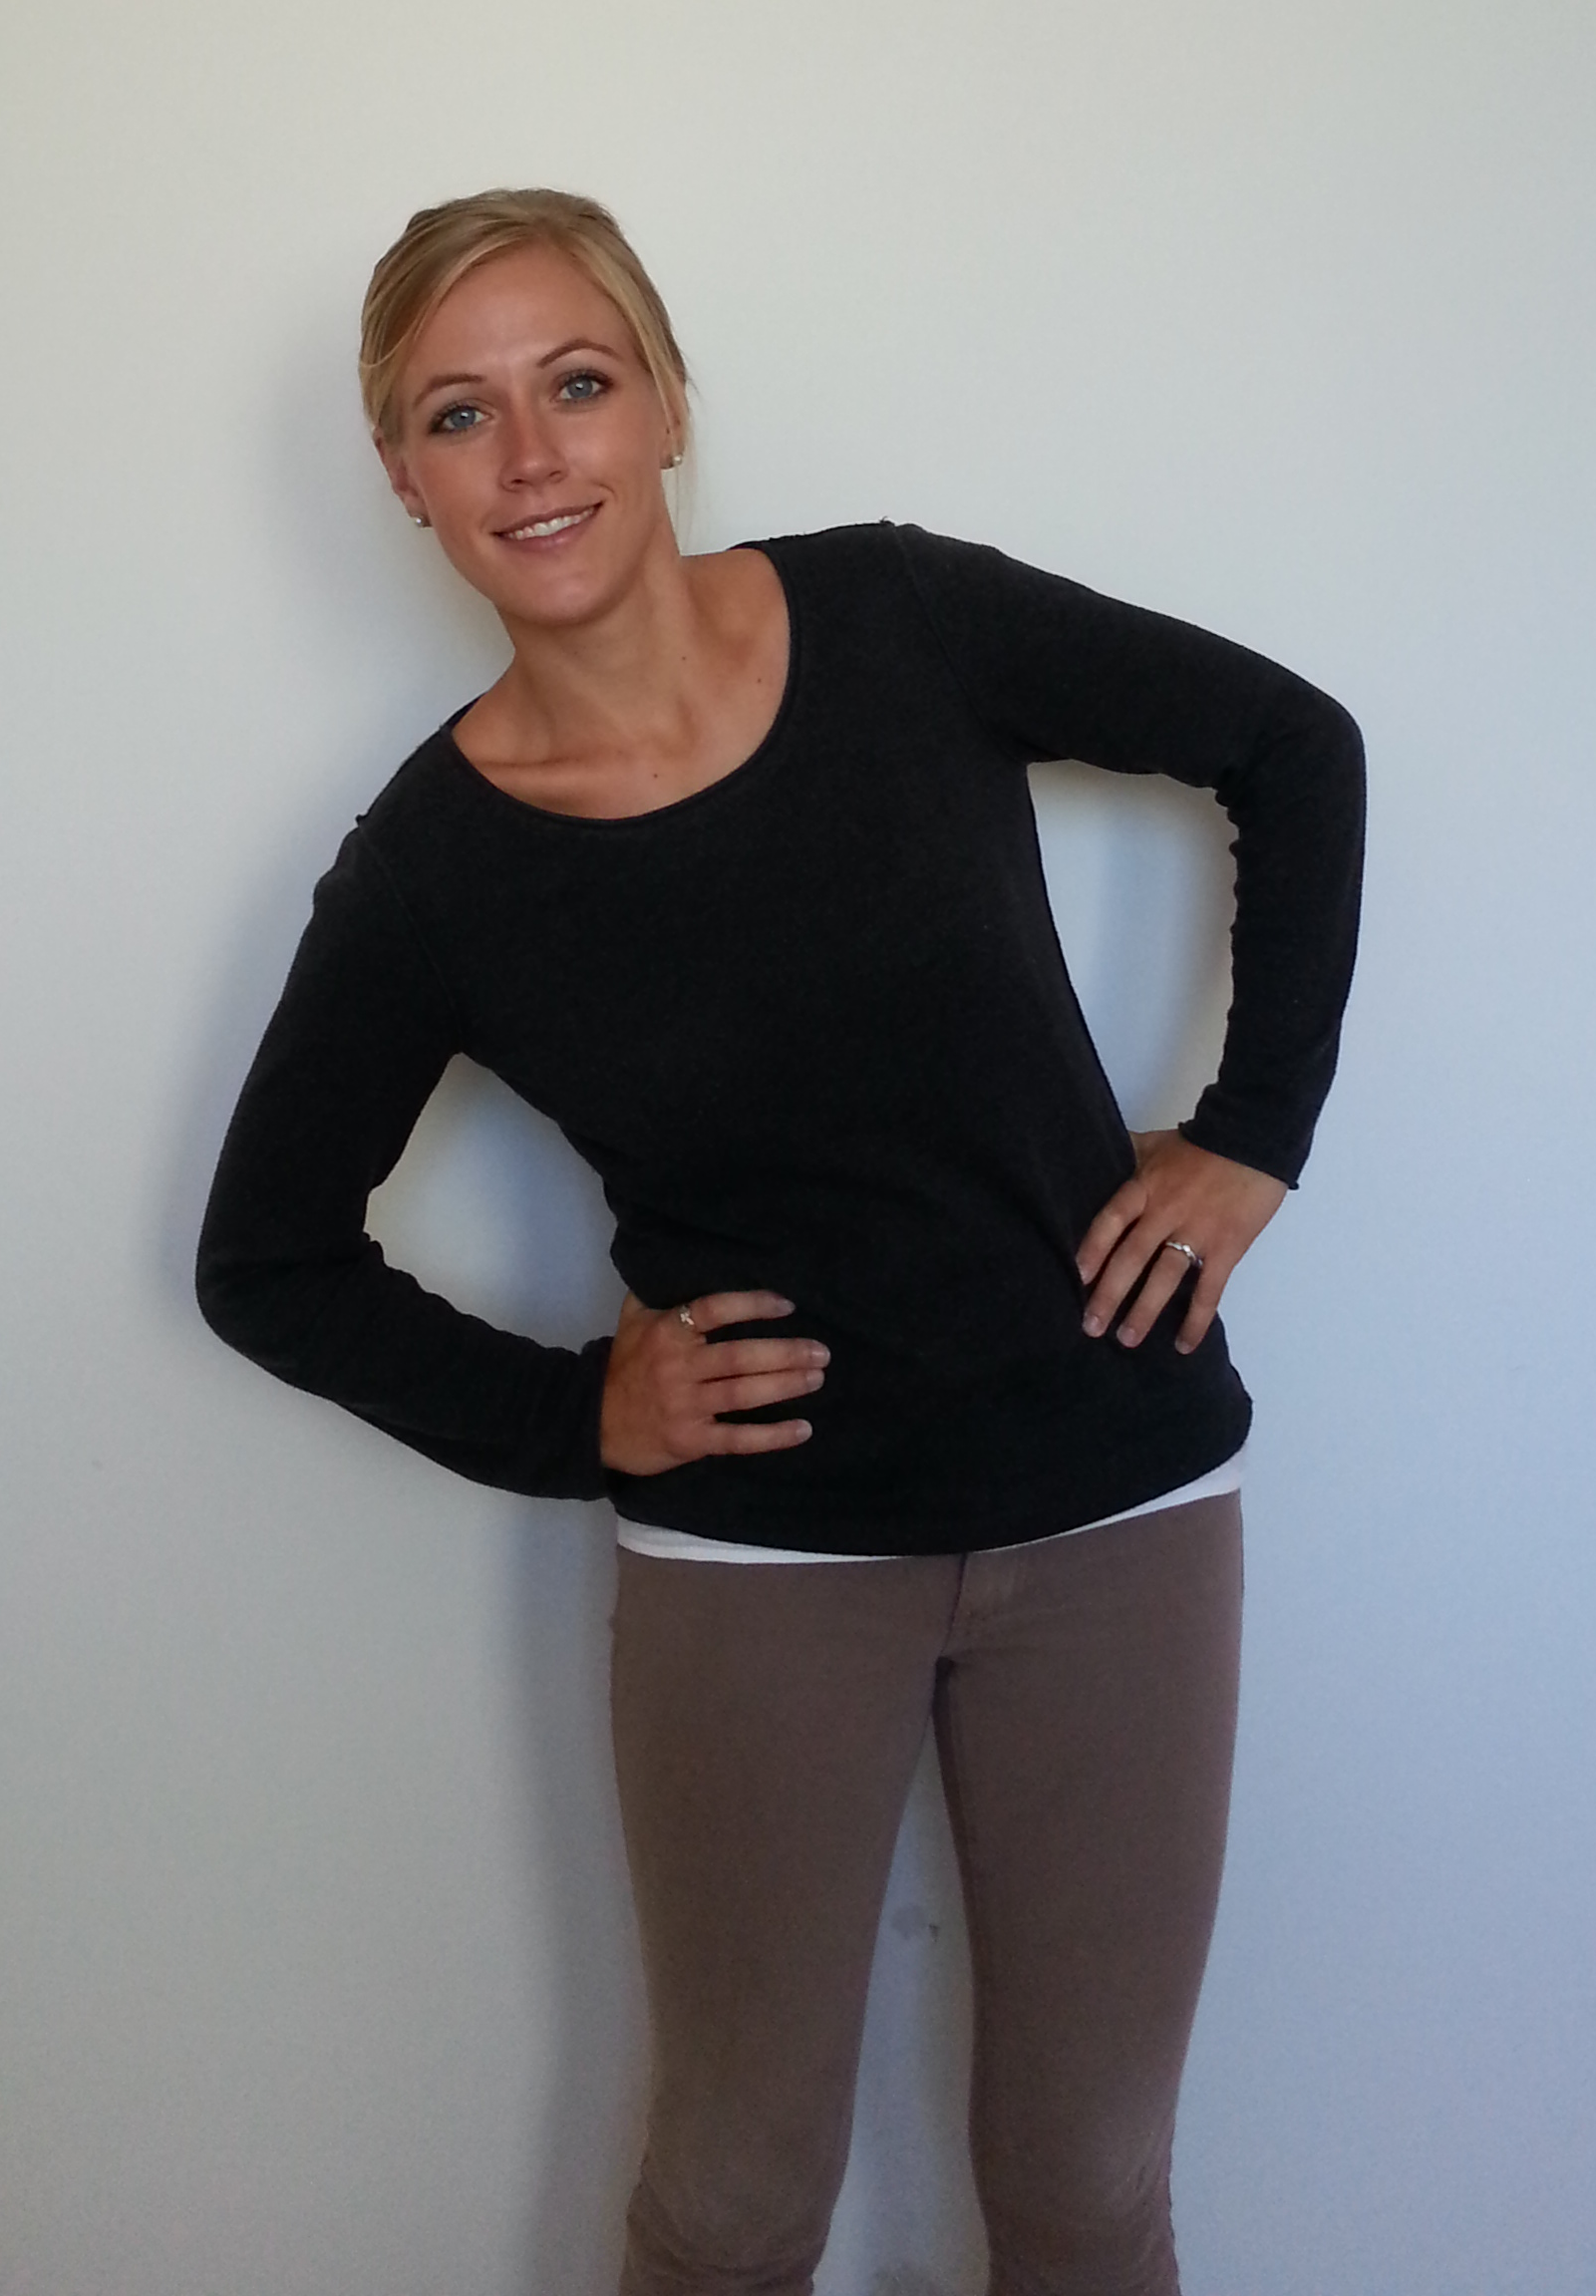
\includegraphics[width=110mm]{mia_bodytilt.png}
%\caption{BodyTilt \label{overflow}}
%\end{figure}

\begin{figure}%
    \centering
    \subfloat[BodyTilt]{{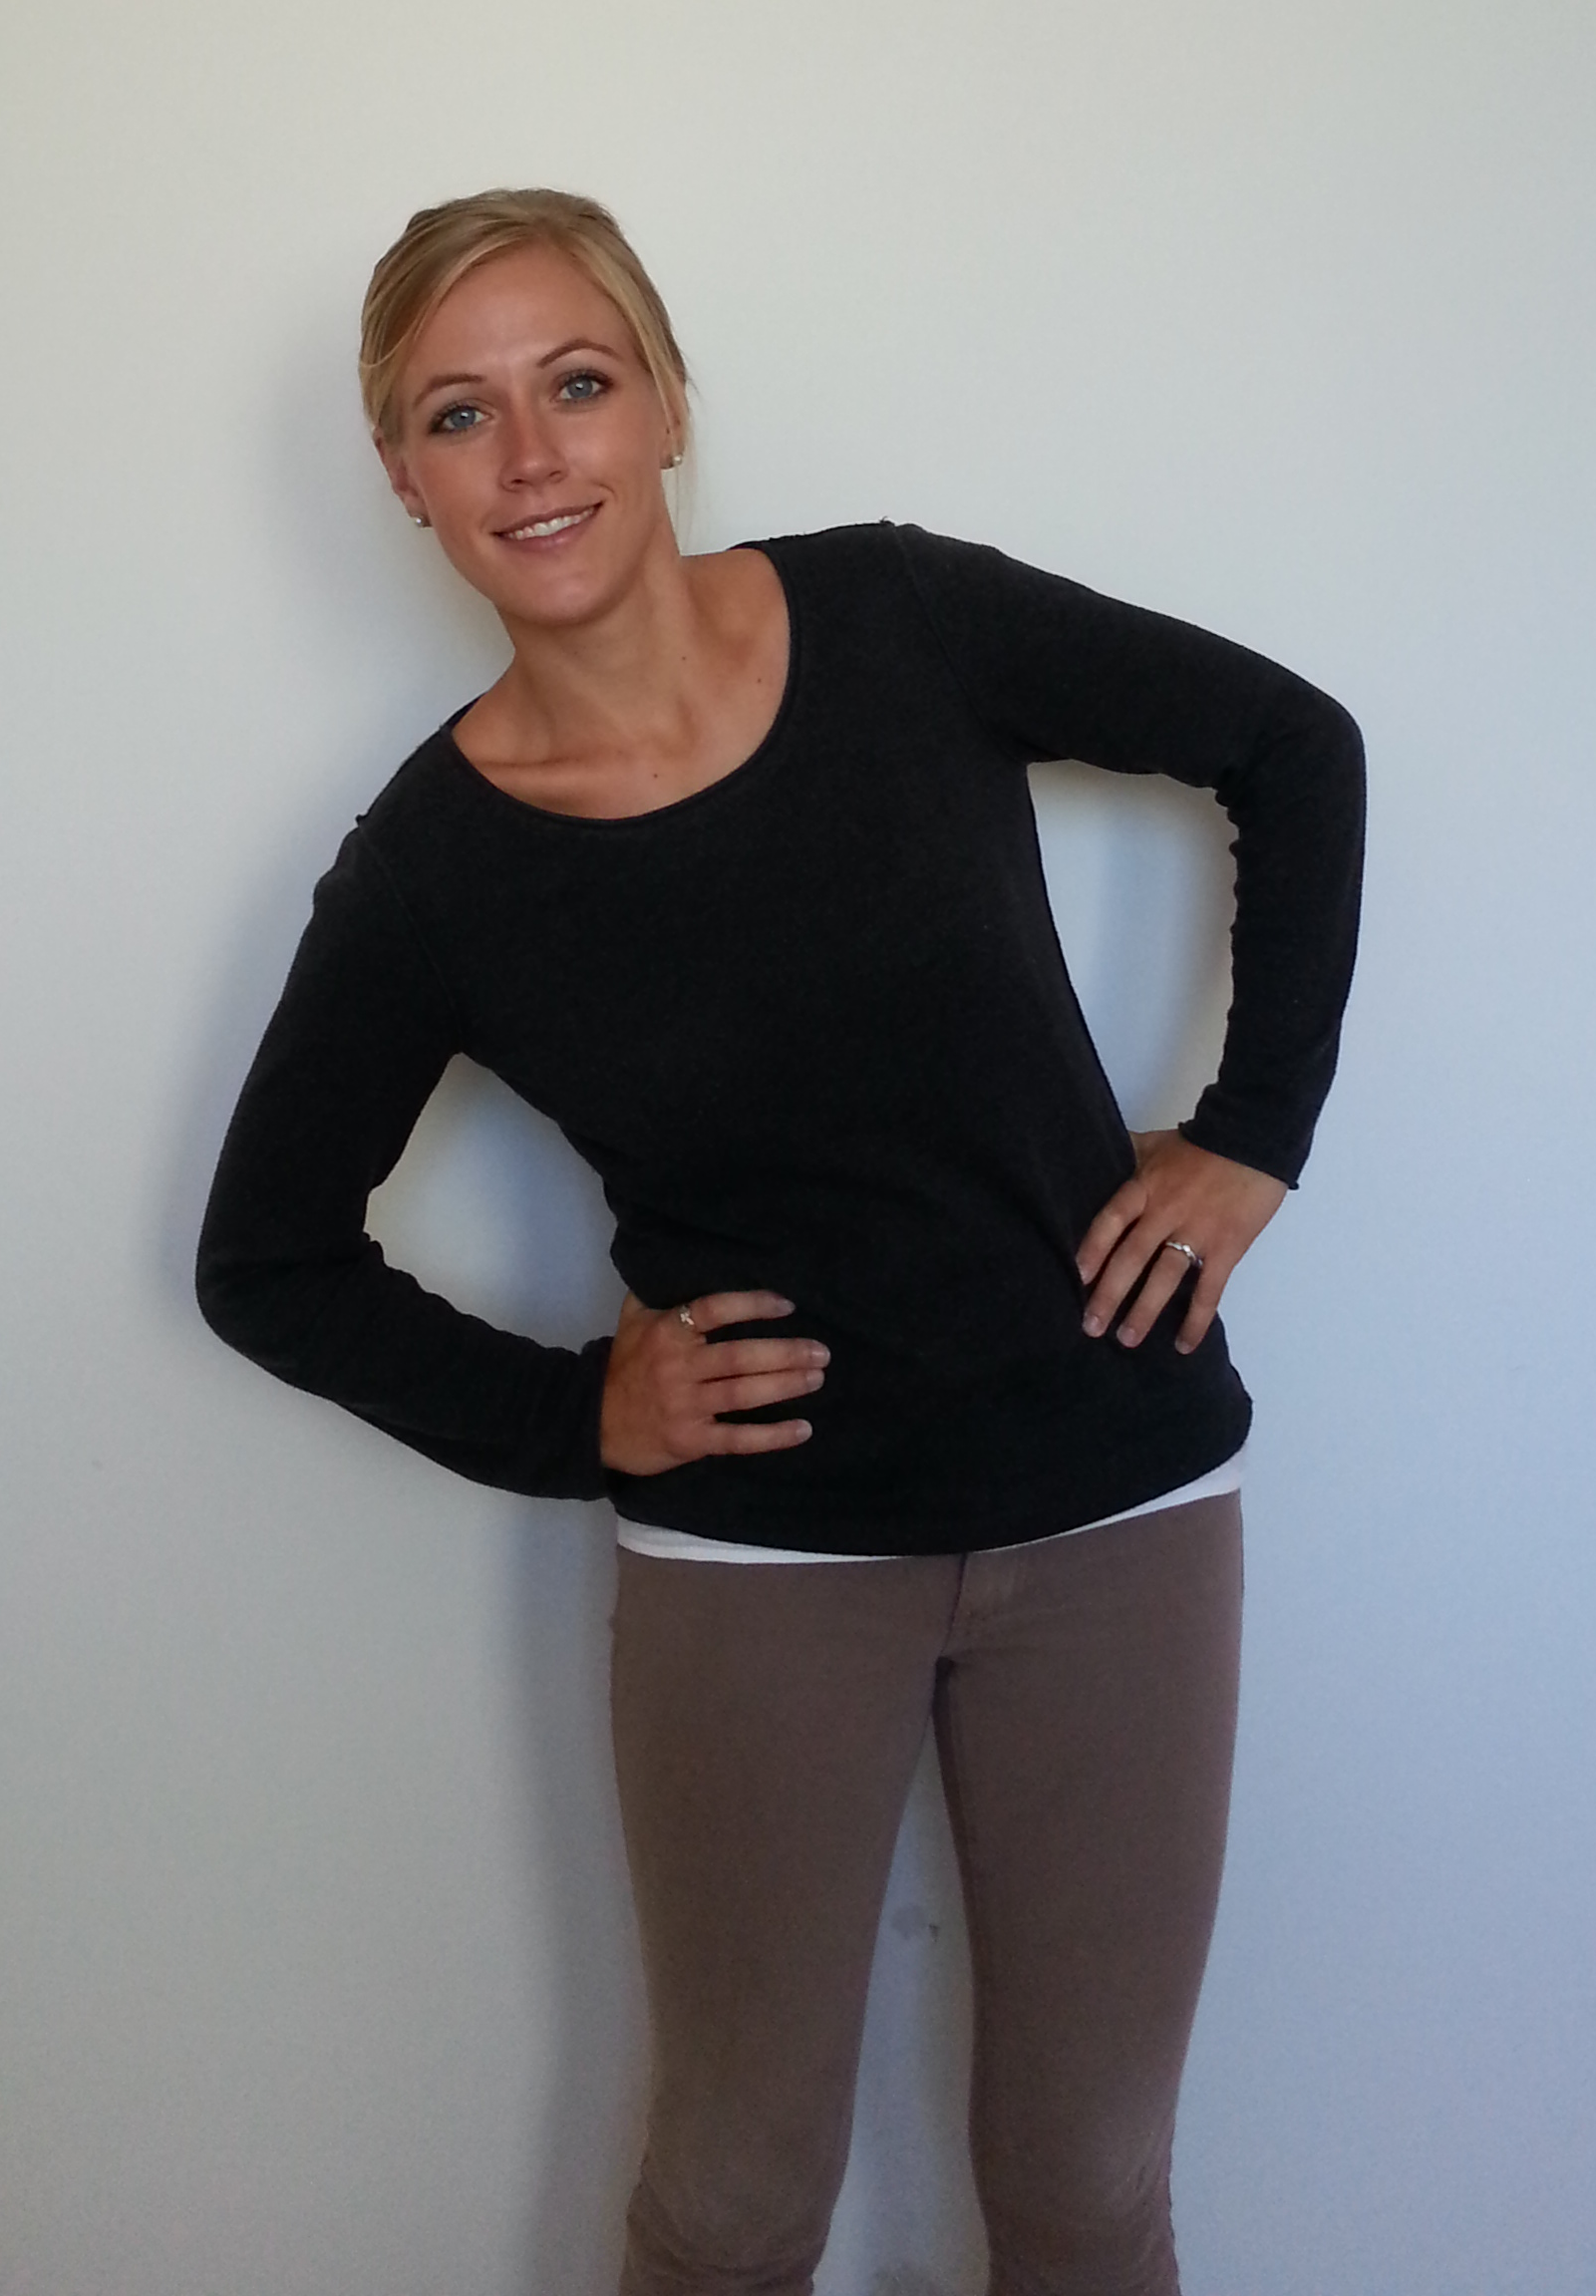
\includegraphics[width=5.5cm]{mia_bodytilt.png} }}%
    \qquad
    \subfloat[HandPoint]{{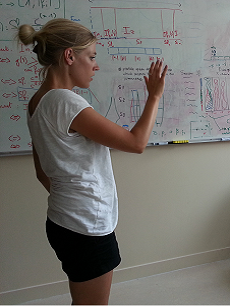
\includegraphics[width=5.5cm]{mia_handpoint.png} }}%
    \caption{Hammer and Planks movement type}%
    \label{fig:movement_type}%
\end{figure}


Before each session, the healthcare professionals will set the number of objects (enemies, bonuses, obstacles), activity duration and repetition, as well as area in which the objects can appear. Therefore he can adjust the difficulty of the game for different session.


\section{Target User Questions}

A traditional Hemiplegic therapy routine usually involved the therapist ordering a patient to perform several movement repetitively \cite{rahman}. By the end of the session, the therapist will analyse how the patient has performed based on the quality of movement as well as how the patient has progressed compared to the previous session. Based on this analysis, the therapist will then configure a new routine to further the patient's progress, if needed.

However, by using a game to facilitate the therapy, it is difficult to monitor how often the patient has moved his/her arm, to which direction and to which objects this movement is associated. Based on this reason, I identified 5 types of questions usually inquired:

\newcommand{\subscript}[2]{$#1 _ #2$}	
\begin{enumerate}[label=(\subscript{Q}{\arabic*})]
\item For a given session, to which direction (right/left) the player moved more? \label{q1}
\item For a given session, how does the player perform based on the number of objects collected, avoided, or killed with respect to the area of the movement?\label{q2}
\item For a given session, how does the player perform based on the number of objects collected, avoided, or killed with respect to the area of movement and the speed in which the game is played?\label{q3}
\item For a given patient, has he/she has improved in the game overtime?\label{q4}
\item For a given patient, has he/she has improved in a certain area overtime?\label{q5}
\end{enumerate}

\section{Visualization Requirements}

The gameplay of each game session is logged in a json file which contains information of the player, game setting, and every events (i.e. enemy killed, bonus collected, etc.) happened in the game. Based on these information and the question defined in the previous section, the tasks can be grouped into: task related to a session for a particular player (Task 1) and task related to the summary of a player which concerns all sessions (Task 2). The following are the tasks defined for each task group:
\newcommand{\task}[2]{$#1 #2$}
\begin{enumerate}[label=\textbf{(\task{T1.}{\arabic*})}]
\item \label{t11} visualize and compare the number of events of an event type at a given x area \ref{q1}\ref{q2}.
\item \label{t12} compare the number of events for different event type at a given x area  \ref{q1}\ref{q2}.
\item \label{t13} visualize and compare the number of events of an event type and its screen speed at a given x area \ref{q1}\ref{q2}\ref{q3}.
\item \label{t14} compare the number of events for different event type and its screen speed at a given x area \ref{q1}\ref{q2}\ref{q3}.
\item \label{t15} select and visualize the number of events for a certain object at a given x area \ref{q1}\ref{q2}.
\item \label{t16} select and visualize the number of events and its screen speed for a certain object at a given x area \ref{q1}\ref{q2}\ref{q3}.
\end{enumerate}

\newcommand{\test}[2]{$#1 #2$}
\begin{enumerate}[label=\textbf{(\test{T2.}{\arabic*})}]
\item \label{t21} visualize and compare the number of events of an event type among each session for one patient \ref{q4}\ref{q5}.
\item \label{t22} compare and navigate the number of events among different event type in a certain x area among each session for one patient \ref{q4}\ref{q5}.
\item \label{t23} select and visualize the number of events of a certain event type in a certain x area among each session for one patient \ref{q4}\ref{q5}.
\item \label{t24} visualize and compare the distribution of certain number of events of an event type over x area among each session for one patient \ref{q4}\ref{q5}.
\item \label{t25} compare and navigate the distribution of certain number of events among different event type over x area among each session for one patient \ref{q4}\ref{q5}.
\item \label{t26} select and visualize the distribution of certain number of events over x area for a certain event type among each session for one patient \ref{q4}\ref{q5}.
\item \label{t27} extract and visualize similar pattern of number of events over a certain x area and sessions for one patient \ref{q4}\ref{q5}.
\end{enumerate}

\chapter{Related Works}
\label{chap:related}

There has been several serious game for hemiplegic rehabilitation developed in the last few years. Similar to Hammer and Planks, these games also has some visualization feature which shows how the player performed so that the therapist is able to make the correct diagnosis. Thus, in this chapter, I first review some of these visualization. Then, since the nature of the input data is time series and movement data, I present some work in visualization which are related to this type of data.

\section{Visualization of Serious Game Result} 

Game result visualization is an integral part of a serious game used for rehabilitation since it's the feature which influence the accuracy of therapist analysis. Most serious game have an analytic feature, however the type of analysis presented depends on the nature of the game and the framework used in the rehabilitation. Therefore, for the purpose of this thesis, I only focus on reviewing serious game which are directed to hemiplegic patients rehabilitation.

In his paper, \cite{rahman} present a rehabilitation framework for hemiplegic patients which combines the use of Kinect and LEAP\footnote{\url{https://www.leapmotion.com/product/desktop}} hand-tracking devices. These devices are attached to a 3D based game environment which was set to accommodate a set of primitive therapy motion such as forearm pronation/supination, shoulder and hip joint adduction/abduction, etc. Similar to Hammer and Planks, one of the game used in the framework requires user to navigate a plane by moving the hand to the right and left (hand-elbow flexion-extension). The recorded movement is then presented in line chart depicting the range of axis of elbow joint (180 degrees when fully extended and 20 degrees when fully flexed) over number of frames captured. Similarly, current visualization in Hammer and Planks also uses line chart to show average body movement over time. At first, line chart is used to represent Hammer and Planks gameplay, however in the end this approach is abandon since it's not intuitive enough. Details of this attempt can be found in chapter 4.

\begin{figure}
\centering
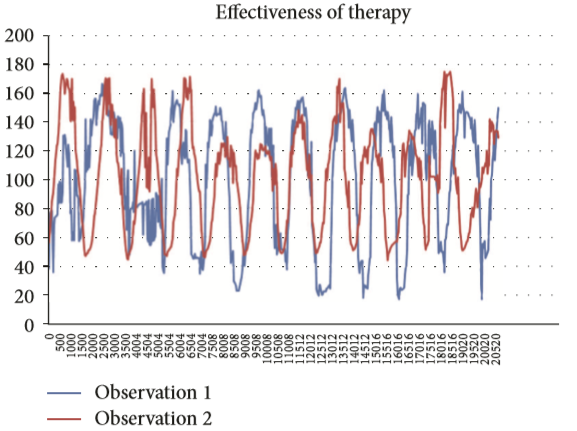
\includegraphics[width=110mm]{rahman_viz.png}
\caption{Visualization used in \cite{rahman} depicting the degree of forearm movement overtime}
\end{figure}

\begin{figure}
\centering
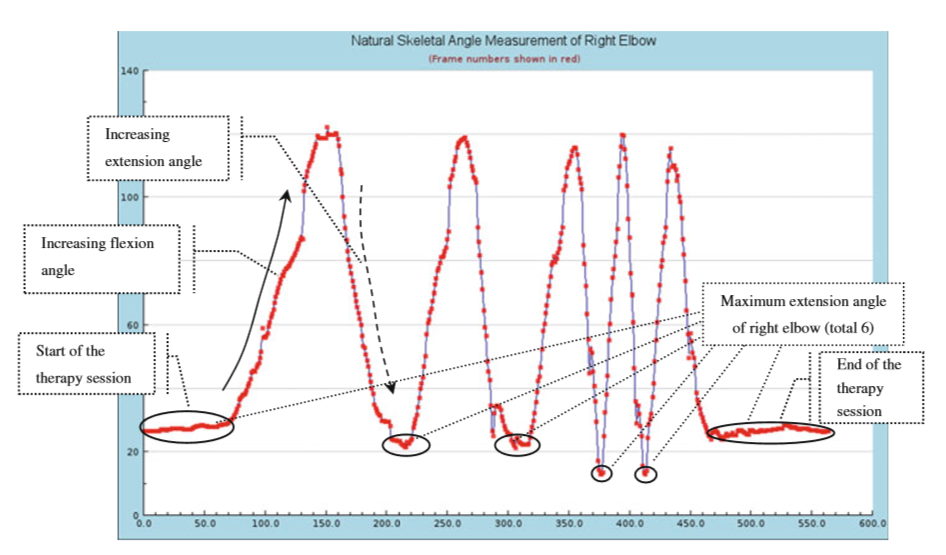
\includegraphics[width=150mm]{rahman2_elbowangle.png}
\caption{Visualization used in \cite{rahman2} depicting the speed of movement (m/s) of forearm overtime}
\end{figure}

In \cite{green}, a virtual reality rehabilitation system for children with hemiplegia was developed using TUI\footnote{\url{https://en.wikipedia.org/wiki/Tangible_user_interface}}. The game itself is displayed on LCD and the player interact with the game by placing the TUI on top of moving targets shown on the LCD. In this system, performances are measured by speed, accuracy and trajectory(mean movement efficiency). However, unlike \cite{rahman}, this system doesn't provide an interface in which therapist can analyse the gameplay.

Similar to Hammer and Planks, \cite{rahman2} introduced a framework which uses Kinect attached to Second Life\footnote{\url{http://secondlife.com/}} serious game environment. The mission of the game is to follow a set of movement that have been configured beforehand by the therapist. During the game, the movement of each body joint  is recorded and saved in Session Recorder. Afterwards, a Kinematic Analytic component will process this data and visualize the quality of improvement metrics of each body joint movement. Each metric is visualized with a dotted line chart over time as shown below. Even though it's possible to  see which line curve indicate an elbow flexion or extension, the therapist needs to count the number of the curve manually. This is not very efficient when the session is longer and there are more curve to count.

\section{Visualization of Time Series Data}

Since one of the requirement of the interface is to have the information of movement evolution over time, it is interesting to review how a time series data is usually visualize. \cite{aigner} discuss at length about the techniques of time series data visualization. This section, reviews some of these interesting techniques.

Considering that the recorded gameplay data contains spatial information (location of an event happened on the screen), some of the reviewed techniques are concerning visualizing spatio-temporal data. \textbf{Flow Map} depicts movements of object over time. Object movements are usually represented by directed trajectories over spatial space(i.e: map) with different color, width, angle of trajectories represent additional information. In order to overcome overlapping trajectories for huge amount of data, usually aggregation techniques (clustering, self organizing map, etc.) are introduced to group similar data point. Figure 3.3 shows an example of flow map depicting photographers movement between cities in Germany \cite{adrienko}. In this case, the aggregation considers three parameters: initial location, destination location, and time period in which the movement happened. Trajectories width indicate the number of photographers who move between the cities. Another visualization technique worth to mention is \textbf{Spatio-Temporal Event Visualization} which uses the space-time cube concept. In this concept, the x and y axis usually represent two spatial dimension while the third axis represent temporal dimension. The events are then represented as graphical objects which are mapped to the space-time cube location. Different events attribute can be represented in different size, colors, shape, or texture. Figure 3.4 shows space-time cube which depict convective clouds \cite{turdukulov}, human health \cite{tominski} and earthquake events \cite{gatalsky} from left to right. As we can see, the  spatial dimension of the left chart is area in pixel while the middle and right chart is a map. The events on the chart are represented with sphere objects with different color and different sizes. Even though space-time cube can portrays the spatio-temporal data, it has some downside. When there are too many events, occlusion is inevitable. It should be coupled with an appropriate interaction technique to allow users see the data from different perspective.

\begin{figure}
\centering
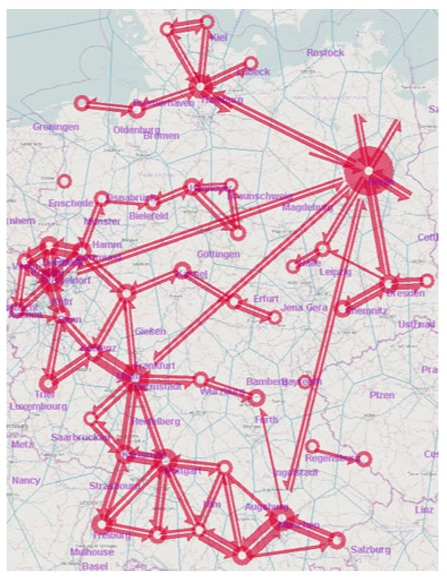
\includegraphics[width=90mm]{aigner_flowmap.jpg}
\caption{Flow Map}
\end{figure}

\begin{figure}
\centering
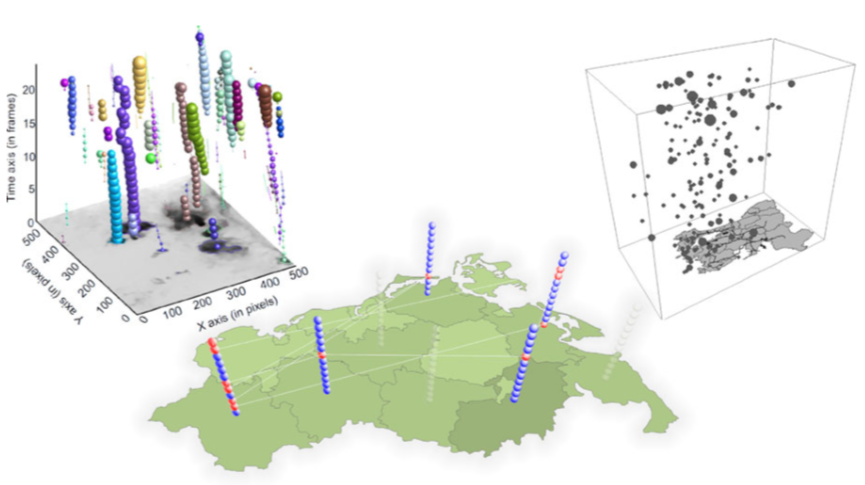
\includegraphics[width=150mm]{aigner_spatiotemporaleventviz.png}
\caption{Spatio-Temporal Event Visualization}
\end{figure}

One example of time-series visualization technique which doesn't concern spatial data is Theme River. First introduced in \cite{havre}, Theme River is used to visualize thematic changes over time of document collection. Each theme is represented as different colors which flows from left to right with different width over different time point. The width depicts theme strength over temporal axis. The purpose of this technique was to easily understand the evolution of theme strength over time. Figure 3.5 shows an example of Theme River representation of 1990 Associated Press newswire data. It can be seen on the chart that the theme baghdad, saddam, iraq, and kuwait are gaining strength  around the time Iraq invaded Kuwait on August 2, 1990. By following the flow of a certain color (theme) we can easily see the changes in theme strength and associate it with the events that affects the changes. Theme River should be supported with interaction techniques which allow user to rearrange river positioning over horizontal axis. 

Consequently, the Theme River technique is chosen due to its ability to show evolution of a certain data variable over time. Further details on the implementation can be found on Chapter 4.

\begin{figure}
\centering
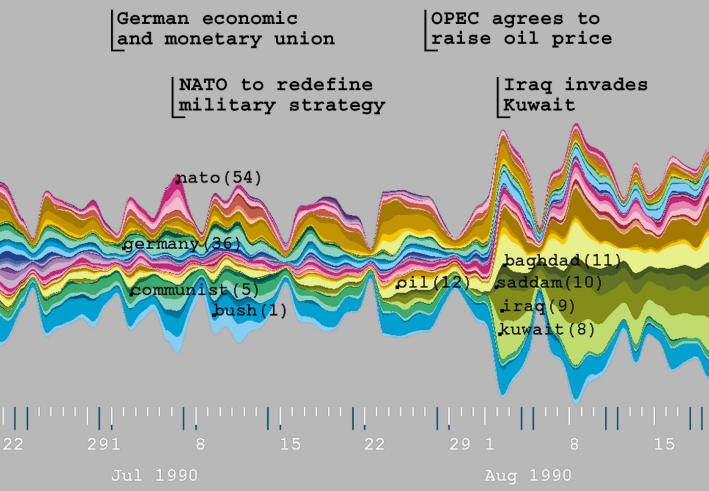
\includegraphics[width=150mm]{havre_themeriver.png}
\caption{Theme River}
\end{figure}


\section{Visualization of Movement Data}

Movement data usually represents an object which moves over a certain space \cite{adrienko_book}: data of moving car, birds migration, etc. It's usually recorded as series of location (latitude/longitude, x/y coordinates, etc.) and time. On the other hand, body movement data are recorded as vector representation of human pose \cite{bernard2013} over time. On this section, I first review visualization for movement data in general and then discuss visualization for body movement focusing on visualization for skeleton animation\footnote{\url{https://en.wikipedia.org/wiki/Skeletal_animation)}} data.

There has been numerous method and application developed to analyse movement data. \cite{adrienko} gives an overview on these methods and applications. Movement data for discrete entities are usually represented as linear symbol over a map or space time cube. However, this technique has problem with occlusions for huge amount of data. Therefore, it's usually accompanied with other graph such as time graph. Other solution to this problem is to use clustering on the trajectories. Apart from minimizing the number of trajectories presented on the view at the same time, clustering also help user to find interesting pattern of the movement. Figure 3.6 \cite{adrienko_book} gives an example of trajectories of a single car from gps data over several days. The trajectories are divided by stop duration at least 3 hours and clustered by route similarity represented in different colors. Therefore, it is possible to know which route are often or less taken by car owner.

\begin{figure}
\centering
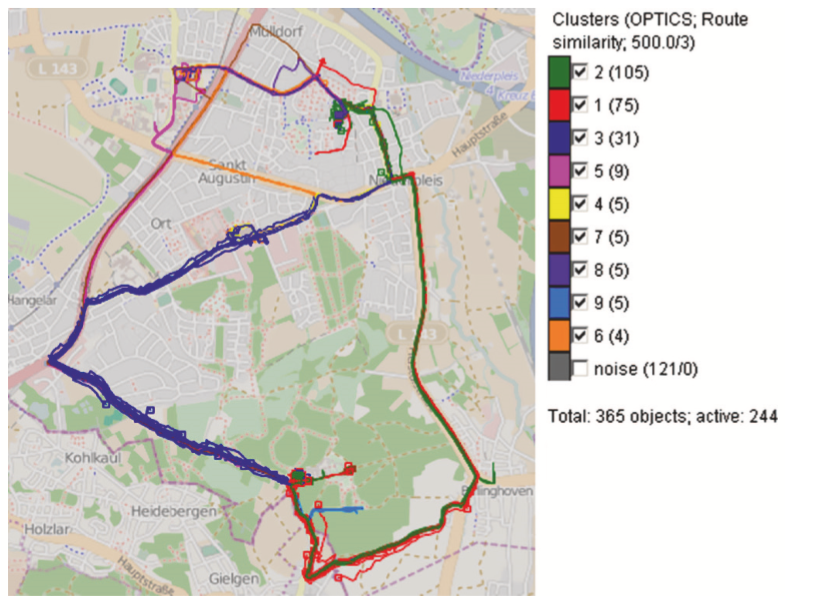
\includegraphics[width=150mm]{adrienko_clustered.png}
\caption{Car Trajectories clustered by route similarity}
\end{figure}

Patterns can also be found by introducing aggregation and generalisation technique on spatial or temporal properties of the movement. For example, the movement data can be aggregated spatially into a discrete grid and for each grid, the number of movement (total or average) happened within the grid can be represented with color or objects in different size. Figure 3.7 \cite{adrienko_book} shows the presence of cars in Milan in certain geographical area (generated with Voronoi tessellation \cite{okabe}) during certain time period. The number of cars in the area is represented with a circle in different size which indicate intensity of traffic. As we can see, there are more traffic between 05-06h (left) compared to 22-23h (right). This is understandable since most people leave work around 5  to 6 pm and are already home at 22-23 pm.

\begin{figure}
\centering
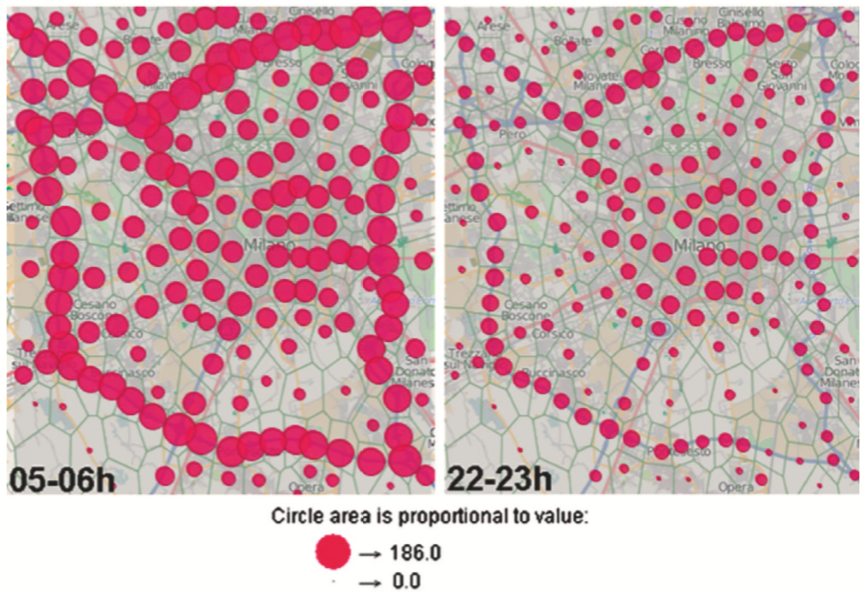
\includegraphics[width=150mm]{adrienko_milan.png}
\caption{Presence of cars in Milan in different time period}
\end{figure}

Recognizing and understanding human movement has many benefits in different application domain: arts\cite{heryadi,raptis}, sports\cite{bernard2013}, healthcare\cite{patsadu}, etc. There are numerous research has been done concerning human movement analysis as discussed in  \cite{gavrila} which surveyed different methodologies and approaches. Most of the methodologies discussed focus on identifying a certain type of movement. On the other hand, to my knowledge, there hasn't been many research which focus on human body movement visualization in which user can explore and analyse a certain data set. 

\cite{chmelik} proposes a system to track and visualize body movement on a virtual environment in real time. In this system, body parts  which desired to be tracked are attached an optical system with twelve infrared cameras. Once user move the tracked body parts, a "motion trail" will be shown in the virtual environment in which then user can manipulate its representation by changing the color, shape, smoothness, etc. These interaction also conducted directly in the virtual environment. Figure 3.8 \cite{chmelik} below shows the motion trail produced in the virtual environment while a user move the tracking device in his hand. On the right is the interface where user can interact with the visualization.

Another approach to visualize body movement is by using color belt \cite{yuko}. In this approach, movement data collected from motion capture system with 11 sensors attached in body joints (Figure 3.9 left) are grouped into 4 limbs movement: Right Arm, Left Arm, Right Leg, Left Leg. Each of the limb representation is arranged in vertical axis sequentially forming a belt. The horizontal axis represents time (from left to right) and the sections represent sets of movement. Limb motions are shown as gradation of red-green colors in this belt by extracting the position and angle of associated body joints data (Figure 3.9 middle). Positive angle is represented with red color, while negative angle is represented with green color. Figure 3.9 (right) shows a color belt and how it is related to the body movement done by a gymnast. The color belt shows the first to fourth movement set. As can be seen in the picture, the gymnast move her leg on the second exercise and the second section on the color belt depicts the movement for right leg and left leg.

\begin{figure}
\centering
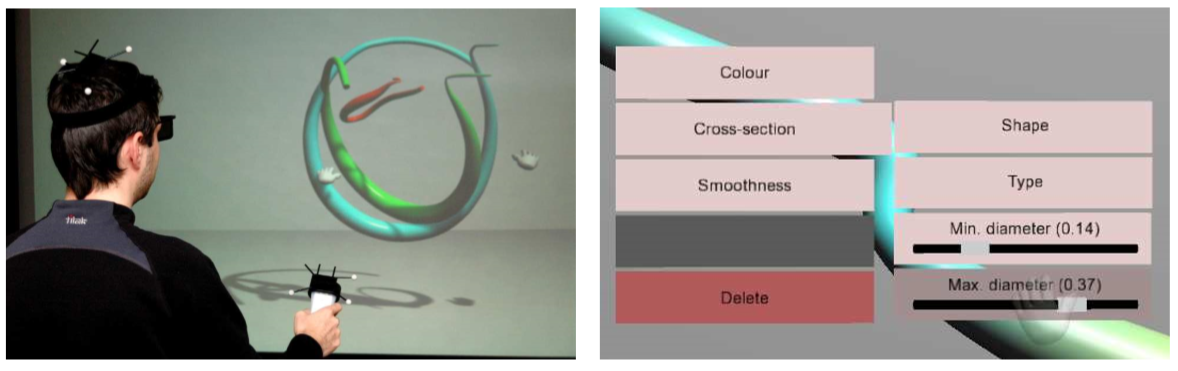
\includegraphics[width=150mm]{chmelik_trail.png}
\caption{Motion Trail}
\end{figure}

\begin{figure}
\centering
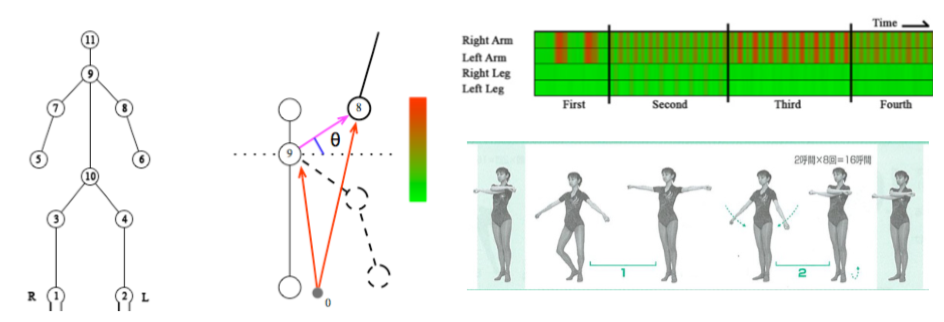
\includegraphics[width=150mm]{yuko_belt.png}
\caption{Color Belt depicting gymnast body movement}
\end{figure}

MotionExplorer\cite{bernard2013} introduced human motion exploratory search using hierarchical aggregation. This approach are directed towards the need to explore huge quantity of motion data and be able to identify interesting sequence of movements. Implemented on database which contains various motions in multiple repetitions, first each human pose data is clustered using k-means algorithm. A pose cluster comprises of a large numbers of similar human pose and is represented as a circular glyph with human stick-figure pose as the centroid and set of pose in the cluster as deviating, transparent figures. The cycle around cluster glyph are colored based on color legend and shows similarity among clusters. MotionExplorer provides 4 views (figure 3.10): (i) \textit{Pose hierarchy explorer} (top left) allows user to explore all available pose cluster in the data sets hierarchically. The pose cluster hierarchy is shown as a dendogram and calculated with a divisive clustering algorithm. The aggregation level is adjustable. (ii) \textit{Motion explorer} (top right) shows sequences between pose clusters at current aggregation level. Human poses are represented as nodes while edges represent motion sequences. Two nodes are connected if there is at least one motion sequence which connects both pose clusters. (iii) \textit{Motion search} interface (bottom right) allows user to input query for a specific motion sequence by inputting start pose and end pose. An interactive search result is provided where user can explore each style variations. The interface is divided into 4 parts: start pose field, search result field, end pose field and pose bundle animation. A user can make search query by choosing/dragging a pose cluster to the start and end pose field. The resulting motion sequences are then shown in the search result field on the granularity of a single human pose. (iv) \textit{Pose color mapping} (box on bottom left) is a color legend related to each pose cluster. The color grid is built using SOM algorithm trained with all feature vectors in a vector quantization scheme. By clicking one of the clusters in the color legend, the aggregation level will be adjusted to the granularity level of the selected pose cluster. Each visualization window is linked. When user changes the aggregation level in the pose hierarchy explorer, the motion explorer is automatically adjusted to the new aggregation level. When user clicks on one of the clusters in the color legend, the system automatically adjust the aggregation level to the same granularity of the selected cluster. If a cluster in one of the view is selected, then the same cluster pose is also highlighted in every view. 

\begin{figure}
\centering
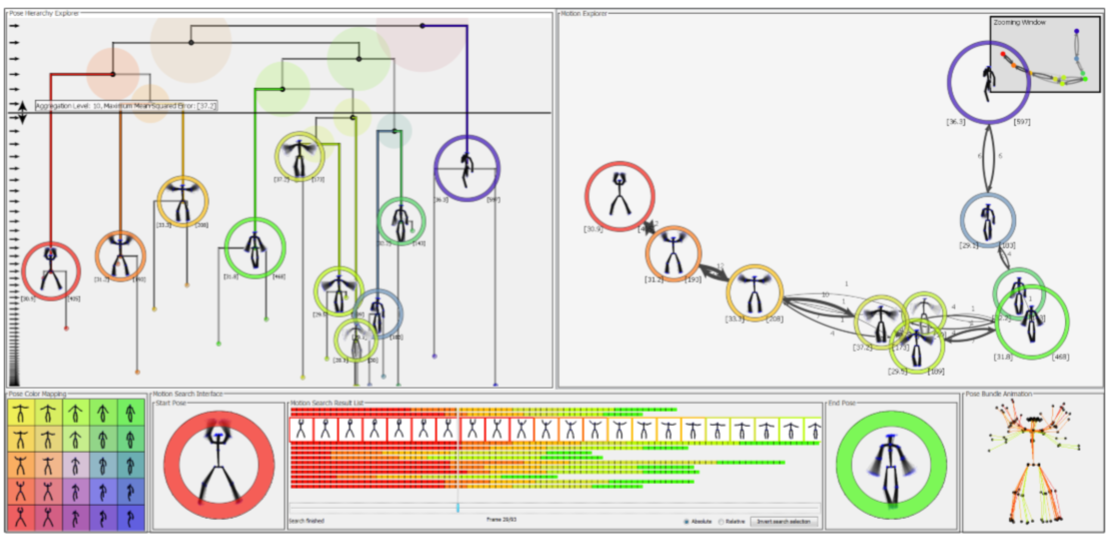
\includegraphics[width=150mm]{bernard_motionexplorer.png}
\caption{MotionExplorer interface}
\end{figure}

\section{Data Visualization Tool}

The popularity of data visualization has been supported with the development of a lot of data visualization tool. To support the development of the interface in this thesis, the survey is focused on tools which allows creation of different visualization technique without restriction of a ready made template or certain chart type. 

One of the tools surveyed is D3\cite{bostock}. \textbf{D3} or Data-Driven Documents is a javascript library which allows user to create desired visualization either the standard one (bar, line, scatter plot, etc.) or the customized one (limited only by one's creativity) in 2D. Built by incorporating HTML5, CSS, and SVG standards, D3 enables user to load data in various format(.json,.csv,.txt, etc.)\footnote{\url{https://github.com/mbostock/d3/wiki/API-Reference}} and present it as a chart. The various functionality offered by D3 and its detailed API documentation has encourage a lot of people to explore it. This resulted in numerous amount of D3 demo online which can be a good reference source for new user\footnote{\url{http://techslides.com/over-2000-d3-js-examples-and-demos}}.

\begin{figure}
\centering
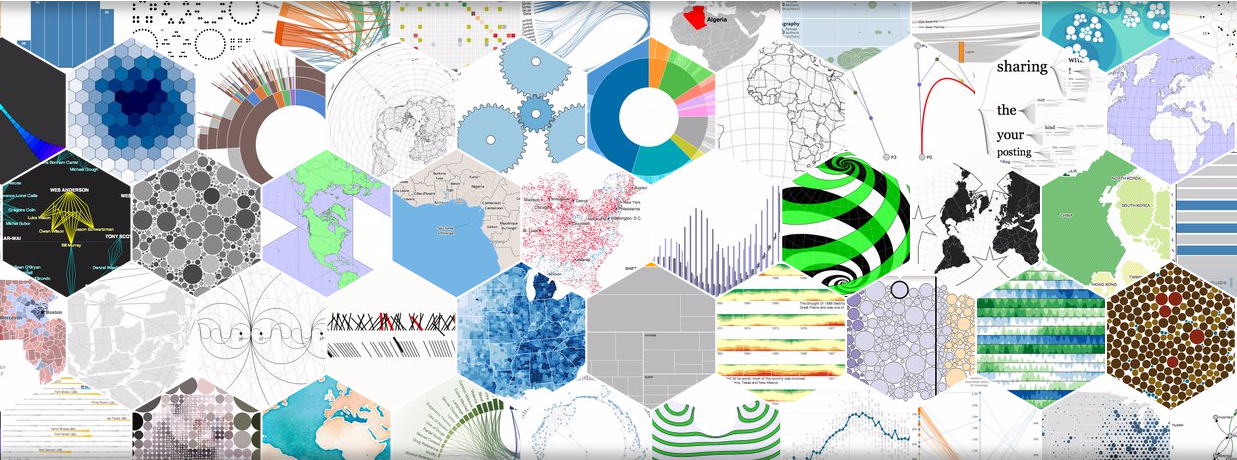
\includegraphics[width=100mm]{d3js.png}
\caption{Some of visualizations developed with D3.js}
\end{figure}

\begin{figure}
\centering
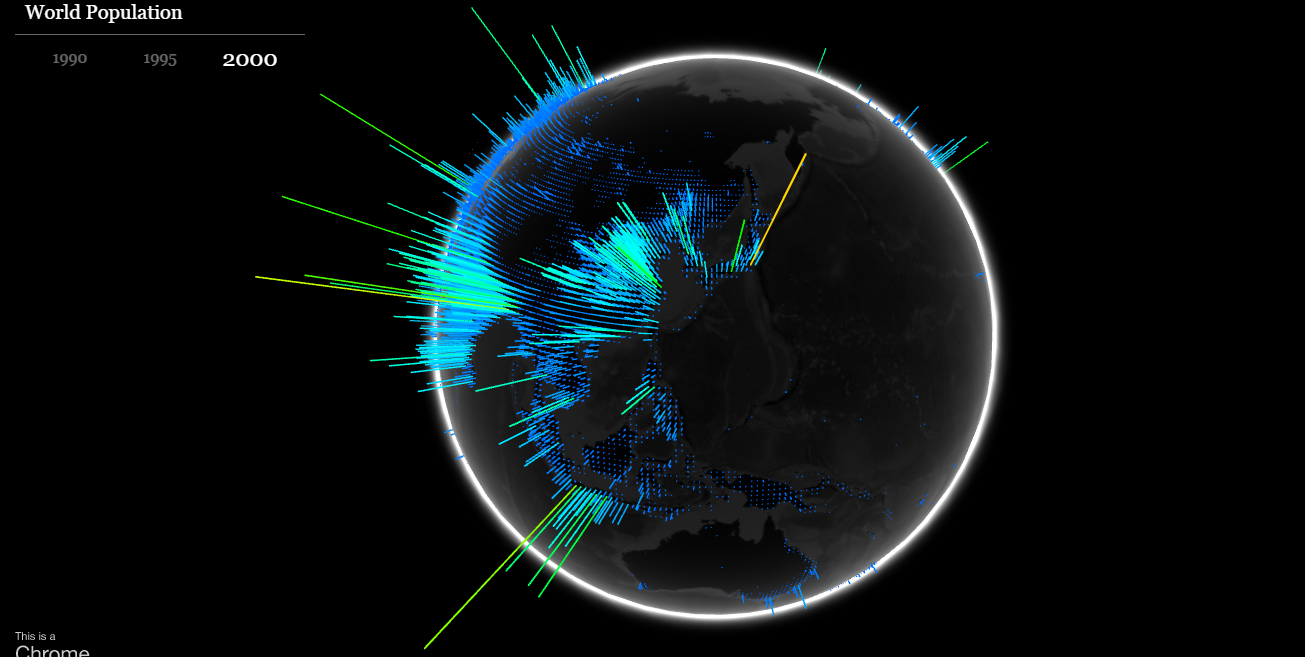
\includegraphics[width=100mm]{threejs.png}
\caption{3D visualization of world population developed in Three.js}
\end{figure}

Another interesting visualization tool reviewed is Three.js. Similar to D3, Three.js is a javascript library. However, Three.js is aimed to provide support for 3D visualizationwith minimal complexity\footnote{\url{https://github.com/mrdoob/three.js/blob/master/README.md}}. The features\footnote{\url{https://github.com/mrdoob/three.js/wiki/Features}} offered by Three.js allows user to develop 3D visualization on WebGL supported web browser without having to install any third party application. Shown in Figure 3.12 visualization of world population on a globe. User can turn the globe around to explore certain area of the world.

Considering the visualization requirement identified in the previous chapter as well as the features offered by D3, consequently D3 is chosen as the tool for interface development.





\chapter{Data Abstraction}

In this chapter I discuss the design of data structure and clustering technique used to support the visual requirement. First, an overview of the input data generated from the game will be explained. Then a description on how this data is extracted to be the input of the visualization interface will be given. Finally, a clustering algorithm selected to be used in the visualization will be discussed.

\section{Game Events Structure}
\subsection{Event Category}
The goal of Hammer and Planks game is to kill all of the enemies while avoiding any attack from the enemies and obstacles\cite{diloreto}. Along the way, player can also catch bonuses to increase their score. Based on these, I identify three different objects within the game: Enemy, Bonus, and Obstacle. For each of these object, there are certain events associated. Each event which happened during the gameplay is recorded in the log file with the following information: event type, timestamp, object id, and location. In total, there are 8 event types:
\newcommand{\events}[2]{$#1 _ #2$}	
\begin{enumerate}[label=({\arabic*})]
\item Catch: when a bonus is catched
\item Miss: when a bonus is missed or player's attack on enemy is missed
\item Dodge: when an obstacle is avoided
\item Collision: when the player's boat collide with an enemy or obstacle
\item Kill: when an enemy is destroyed by player's boat
\item Hit: when the player's attack hit an enemy
\item Hurt: when the enemy's attack hit player's boat
\item Miss: when the enemy's attack missed player's boat
\end{enumerate}

Based on the level of impact of each event to the user's boat, we characterize the event by assign it with Positive, Neutral, or Negative as shown in the following table:
\begin{table}[h]
\begin{center}
    \begin{tabular}{| l | l | l | l |}
    \hline
    Events & Bonus & Obstacle & Enemy \\ \hline
    Positive & catch & - & kill,hit\\ \hline
    Neutral & miss & dodge & miss\\ \hline
    Negative & - & collision & hurt, collision\\
    \hline
    \end{tabular}
    \caption {Event Type grouping}
\end{center}
\end{table}

\subsection{Game World Coordinates}
Each object and event in the game are assigned with 3D location coordinates. An \textit{x} axis of this coordinate indicate horizontal axis of the screen. However, \textit{y} axis indicate vertical axis in the game world which means -\textit{y} is a location under the sea and +\textit{y} is above the sea. \textit{z} axis indicate vertical axis of the screen. The visualization uses the x axis to represent body movement over horizontal axis and z axis to calculate screen speed as explain in the following sub section.

\subsection{Screen Speed}
In the game, a big number of positive events indicate a good player's performance. However, it is important to consider whether the events happened when the player's boat move fast or slowly \ref{t14}\ref{t16}. Getting all the bonuses while moving fast requires precise hand/body movement which indicates improvement in rehabilitation process. Boat speed while navigating the sea is basically the speed in which the screen scroll($\upsilon_{scr}$). This is calculated by identifying the location(apparition z coordinate $\theta_{apr}$) and time (apparition time $\textit{t}_{apr}$) of an object when it first appear on the screen, and location(event z coordinate $\theta_{evt}$) and time(event time $\textit{t}_{evt}$) when an event happened on that object.

$$ \upsilon_{scr} = \frac{\theta_{evt}-\theta_{apr}}{\textit{t}_{evt}-\textit{t}_{apr}} $$

\section{Clustering}

In understanding the evolution of movements among different sessions over x-area, it is interesting to see what the common evolution of different section of the x-area\ref{t27}. The idea is to cluster similar distribution of movements (which is represented by events in the game) so that consecutive section which has similar evolution is represented by a single representation. This section explains how the clustering is done. First, a distance function used to calculate the difference between two consecutive section will be presented. Then, a clustering algorithm based on hierarchical clustering which incorporate this distance function will be explained.

\subsection{Distance Calculation}
Let S be a gameplay data set of $n_{ses}$ sessions. S is an ordered list of sections $s_i, 0 \le i < n_{sec}$. Each section contains events occurred on an x-axis unit among all sessions. More precisely, a  section $s_i$ is a sequence of triplets $s_i\lbrack j \rbrack, 0 \le j < n_{ses}$. Each triplet represents data set of a certain game session of a particular section $s_i$. The triplet consists of the number of negative, neutral and positive events. The profile of each section can be represented by a matrix of $n_{ses}$ x 3 dimensions. For instance, the following matrices represents a gameplay with 2 sessions and 3 sections:

\[
\textit{s}_1 = \begin{bmatrix}
  10 & 20 & 6\\
  20 & 5 & 18
\end{bmatrix}
\textit{s}_2 = \begin{bmatrix}
  20 & 40 & 10\\ 
  40 & 10 & 30
\end{bmatrix}
\textit{s}_3 = \begin{bmatrix}
  10 & 20 & 5\\
  16 & 4 & 12 
\end{bmatrix}
\]

In this example, we see that on the left part of the x-axis ($s_1$), the player got 10 negative, 20 neutral and 6 positive events for the first session. He then got 20 negative, 5 neutral and 18 positive events for the second session. On the middle part of the x-axis ($s_2$), on the first session he got 20 negative, 40 neutral and 10 positive events, while on the the second session he got 40 negative, 10 neutral, and 30 negative events.

Since the idea was to aggregate consecutive sections with similar movement pattern, a function to quantify the similarity between two sections is needed. In this case, we quantify the similarity by defining a distance function. Thus, distance equals 0 indicates that both sections are similar, while distance equals 1 indicates that both sections are different. We identified that there are two types of distance need to be considered: (i) how different both sections in term of event types proportion within each section (ii) how different both sections in term of the evolution of each event type throughout the sessions. For instance, with the (i) approach, $s_2$ and $s_3$ are similar, because triplets of each sessions are proportional ([20,40,10] is proportional to [10,20,5] and [40,10,30] is proportional to [16,4,12]). With the (ii) approach, $s_1$ and $s_2$ are similar, because the corresponding event types are proportional ([10,20] is proportional to [20,40], [20,5] is proportional to [40,10], and [6,18] is proportional to[10,30]).

Thus, for each pair of consecutive sequences ($\textit{s}_1$,$\textit{s}_2$) of \textit{S}, distance is defined as weighted sum of (i) and (ii), represented as $\textit{f}(\textit{s}_1,\textit{s}_2)$ and $\textit{g}(\textit{s}_1,\textit{s}_2)$ in the following formula:

$$d(\textit{s}_1,\textit{s}_2) = \alpha\textit{f}(\textit{s}_1,\textit{s}_2) + (1 - \alpha)\textit{g}(\textit{s}_1,\textit{s}_2)$$

Distance function $f(\textit{s}_1,\textit{s}_2)$ is based on a normalized euclidean distance between two triplets of the same session between two consecutive sections. The overall distance of both sections is the average euclidean distance of each triplets pair. To get a value of distance between 0 and 1, each Euclidean distance value is normalized by dividing it with maximum distance $\sqrt{3}$.

$$f(\textit{s}_1,\textit{s}_2) = \frac{\displaystyle\sum_{i=0}^{i < \lvert\textit{s}_1\lvert} \textit{N}ED(\textit{s}_1\lbrack i \rbrack,\textit{s}_2\lbrack i \rbrack)}{ \lvert\textit{s}_1\lvert}$$

$$ \textit{N}ED(\textit{s}_1\lbrack i \rbrack,\textit{s}_2\lbrack i \rbrack) = \frac{\sqrt{\displaystyle\sum_{j \in \{0,1,2\}}(\textit{s}_1'\lbrack i \rbrack\lbrack j \rbrack - \textit{s}_2'\lbrack i \rbrack\lbrack j \rbrack)^2}}{\sqrt{3}}$$

In this first distance function, $\textit{s}_1'$ and $\textit{s}_2'$ represent normalized value of $\textit{s}_1$ and $\textit{s}_2$. Since the first distance is to see the difference of event type proportion in each section, thus the values are normalized by the maximum value of each sessions in each section. In this case, two consecutive sections with different number of events but similar proportion of event type will have distance equals 0.  For example, the matrices presented previously can be normalized into the following matrices:

\[
s_1' = \begin{bmatrix}
  \frac{1}{2} & 1 & \frac{6}{20}\\ 
  1 & \frac{1}{4} & \frac{18}{20}
\end{bmatrix}
s_2' = \begin{bmatrix}
  \frac{1}{2} & 1 & \frac{1}{4}\\
  1 & \frac{1}{4} & \frac{3}{4} 
\end{bmatrix}
s_3' = \begin{bmatrix}
  \frac{1}{2} & 1 & \frac{1}{4}\\
  1 & \frac{1}{4} & \frac{3}{4} 
\end{bmatrix}
\]

Thus, distance \textit{f} of $s_1$ and $s_2$ equals 0.06, and distance \textit{f} of $s_2$ and $s_3$ equals 0.

The second distance function $\textit{g}(\textit{s}_1,\textit{s}_2)$ is based on a normalized euclidean distance between the same event type \textit{j} from different section. The overall distance of both sections is the average euclidean distance of each event type pair. For each event type distance, there are three different distance value defined: (i) if there are no events in both event type pairs, the distance is 0 (ii) if there is at least one event in one section and there are no events in the other section, the distance is 1 (iii) if both event type pairs has any events then the euclidean distance is calculated. Distance (i) and (ii) are defined to isolate empty regions. Thus when both sections are empty, it will be considered similar and will be clustered together. On the other hand, when only one section is empty while the other has some events, it will be considered as different session and therefore will not be clustered together. To get a value of distance between 0 and 1, each Euclidean distance value is then normalized by dividing it with maximum distance $\sqrt{\lvert\textit{s}_1\rvert}$.

$$\textit{g}(\textit{s}_1,\textit{s}_2) = \frac{\textit{g}_0(\textit{s}_1,\textit{s}_2) + \textit{g}_1(\textit{s}_1,\textit{s}_2) + \textit{g}_2(\textit{s}_1,\textit{s}_2)}{3}$$

\[\text{and for } j  \in \{0,1,2\}\text{, } g_j(\textit{s}_1,\textit{s}_2) = \left\{
  \begin{array}{ll}
    0 & \text{ if } \textit{s}_k\lbrack i \rbrack\lbrack j \rbrack=0 \text{ for each } 0 \leqslant j < |\textit{s}_k|\text{ and } \textit{k} \in \{1,2\}\\
    1 & \text{ if } \textit{s}_k\lbrack i \rbrack\lbrack j \rbrack=0 \text{ for each } 0 \leqslant j < |\textit{s}_k| \text{ and } \exists \textit{s}_p\lbrack i \rbrack\lbrack j \rbrack \neq 0,\\
      & k,p \in \{1,2\} \text{, } k \neq p\\
      & \\
	\multicolumn{2}{l}{\frac{\sqrt{\displaystyle\sum_{i=0}^{\lvert\textit{s}_1\lvert} (\textit{s}_1''\lbrack i \rbrack\lbrack j \rbrack - \textit{s}_2''\lbrack i \rbrack\lbrack j \rbrack)^2}}{\sqrt{\lvert\textit{s}_1\rvert}} \text{ otherwise}} 
  \end{array}
\right.
\]

Here, $s_1''$ and $s_2''$ represent normalized value of $s_1$ and $s_2$. In order to compare the evolution of the same event type between consecutive sections, the values are normalized by dividing it with maximum value of each event type in the section. Thus, the matrices presented previously can be normalized into the following:

\[
s_1'' = \begin{bmatrix}
  \frac{1}{2} & 1 & \frac{1}{3}\\ 
  1 & \frac{1}{4} & 1
\end{bmatrix}
s_2'' = \begin{bmatrix}
  \frac{1}{2} & 1 & \frac{1}{3}\\ 
  1 & \frac{1}{4} & 1
\end{bmatrix}
s_3'' = \begin{bmatrix}
  \frac{5}{8} & 1 & \frac{5}{12}\\
  1 & \frac{1}{5} & 1 
\end{bmatrix}
\]

Here, distance \textit{g} of $s_1$ and $s_2$ equals 0, and distance \textit{g} of $s_2$ and $s_3$ equals 0.06. 

\subsection{Clustering Algorithm}
The sections clustering follows Hierarchical Clustering algorithm \cite{maimon} which is a clustering analysis method used to build hierarchy of clusters. In our approach, once distance of each consecutive sections are calculated, two consecutive sections with distance below a specified threshold are then merged. This resulting in a new set of sections. Then, the distance of each consecutive sections of these new set of sections are calculated and again, if the new distance satisfies the threshold, the sections will be merged. This process is repeated until there is no distance falls below the threshold.








\chapter{Visual Mappings And Interactive Functionalities}
This chapter describes different visualizations and interaction methods developed based on the visualization requirements and data abstraction discussed in Chapter 2 and 4. In general, the visualization is divided into two parts: (i) Session Visualization which visualize movement in one particular session (for \textit{T}1.x) and (ii) Summary Visualization which visualize movement over different sessions (for \textit{T}2.x). Both visualization is organized in an application where user can select player and sessions he has played. At first, the earlier version of visualization will be explained. This earlier version is not used in the final version since it's difficult to get any information intuitively. Then, each type of visualization and its interaction used in the final version will be discuss. In the end, the application which encapsulate both visualization will be presented.

\section{Early version of Session Visualization}
The first visualization method chosen to represent \ref{t11} is line chart. In this approach, the x area is shown as a horizontal axis and the number of events shown in vertical axis with the line signify the changes of number of events for different x area unit. In the log file, each event is recorded with distinct 3D coordinate location. The x value from this coordinate is a decimal, therefore visualizing each one of this x value will require a lot of space. To solve this, the events are then grouped by the rounded x value. In Figure \ref{first_linechart} below, Negative events are shown in red line and Positive events are shown in blue line. As we can see, it's possible to know which event type happened more in a certain x unit, however it is difficult to see how big a percentage is it compare to total number of events happened in the same x unit.

\begin{figure}
\centering
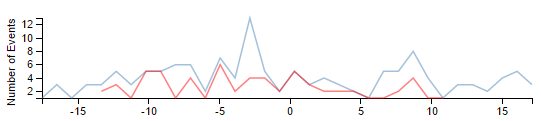
\includegraphics[width=100mm]{linechart.png}
\caption{First visualization version for \ref{t11} using Line Chart}
\label{first_linechart}
\end{figure}

\begin{figure}
\centering
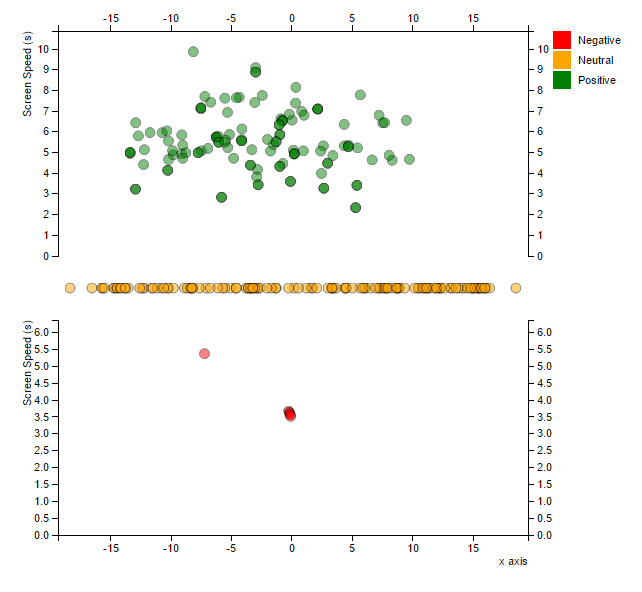
\includegraphics[width=100mm]{scatterplot.png}
\caption{First visualization version for \ref{t12} using Scatter Plot}
\label{first_scatterplot}
\end{figure}

Visualization method chosen to represent \ref{t12} is scatter plot. At first, each event type is presented in three different chart area: top are for Positive events, middle are for Neutral events, and bottom area for Negative events. Similar to the line chart, the x value from the 3D coordinate location are represented in horizontal x axis. However, the vertical axis here represents screen speed. For the scatter plot, each event is shown as a plot in the chart area according to it's x value and screen speed as shown in Figure \ref{first_scatterplot}. Even though similar pattern can be seen on the scatter plot, occlusion problem prevents users to know how many event are actually happened in a certain x area.

\section{Session Visualization}
The Session Visualization shows events within a game session. The requirement can be split into two: (i) knowing the distribution of events and movements (ii) knowing the distribution of events, movements and screen speed. Basically, (ii) is a detailed view of (i). Therefore, there are two chart developed to meet these requirements: stacked area graph for (i) and heatmap for (ii), each of which will be explain in details in this section.

\subsection{Stacked Graph}
Build on layered area graph, Stacked Graph is widely used to visualize evolution of variable over times such as document theme \cite{havre}, box office movie revenue\footnote{\url{http://www.nytimes.com/interactive/2008/02/23/movies/20080223_REVENUE_GRAPHIC.html?_r=0}}, listening history in Last.fm \cite{byron},etc. Stacked Graph is chosen because its ability to show individual value of a variable, the difference between values of different variables as well as the total of overall value. In our approach, instead of using this metaphor to show evolution over time, it is used to show distribution of events over spatial coordinate \ref{t11} as shown in Figure \ref{fig:linear}. Here, the horizontal axis represents x coordinate and vertical axis represents number of events. Each event type is represented as an area with different color: Red (Negative), Yellow (Neutral), and Green (Positive). However, with this approach it is difficult to see the trend for each individual events which is not on the base of the chart. \cite{alan} propose an interactive solution to this problem by sinking the selected category to the horizontal axis. Thus, in our visualization, different layout of stacked graph is provided: 
\begin{enumerate}
  \item Linear (Figure \ref{fig:linear}): zero y axis is used as the baseline, with the stack ordered from the bottom as Negative, Neutral, Positive.
  \item Silhouette (Figure \ref{fig:silhouette}): the graph is centered as in streamgraphs.
  \item Positive (Figure \ref{fig:positive}): zero y axis is located at the top of the chart and is used as the baseline with the stack ordered from the top as Positive, Neutral, Negative.
  \item Neutral-Negative (Figure \ref{fig:neutral-negative}): zero y axis is located in the middle of the chart. Neutral and Positive events are shown on the positive area of y axis and Negative events are shown on the negative area of y axis.
  \item Positive-Neutral (Figure \ref{fig:positive-neutral}): zero y axis is located in the middle of the chart. Positive events are shown on the positive area of y axis, while Neutral and Negative events are shown on the negative area of y axis.
\end{enumerate}

\begin{figure}
\centering
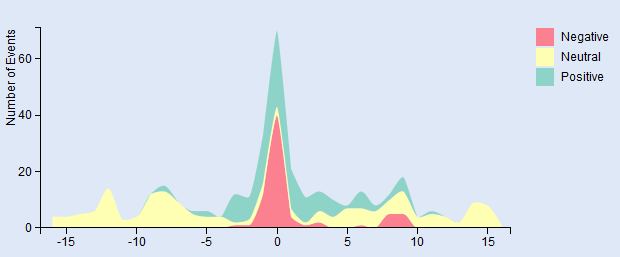
\includegraphics[width=100mm]{stackedgraph_linear.png}
\caption{Stacked Graph with Linear Layout}
\label{fig:linear}
\end{figure}

\begin{figure}[htp] % not h only
\centering
\subfloat[Silhouette]{%
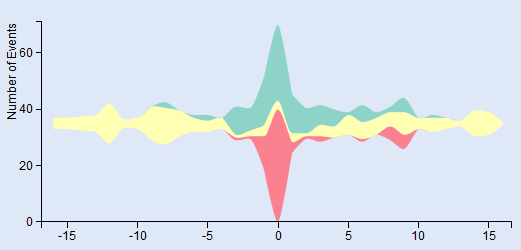
\includegraphics[width=0.4\textwidth]{stackedgraph_silhouette.png}%
\label{fig:silhouette}%
}\hfil
\subfloat[Positive]{%
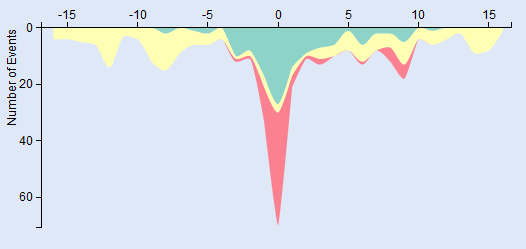
\includegraphics[width=0.4\textwidth]{stackedgraph_positive.png}%
\label{fig:positive}%
}

\subfloat[Neutral-Negative]{%
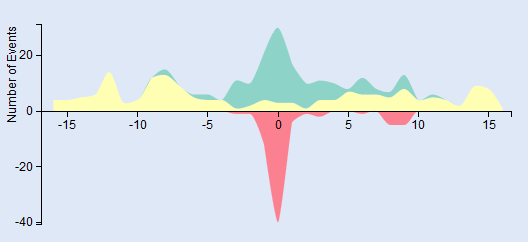
\includegraphics[width=0.4\textwidth]{stackedgraph_neutral_neg.png}%
\label{fig:neutral-negative}%
}\hfil
\subfloat[Positive-Neutral]{%
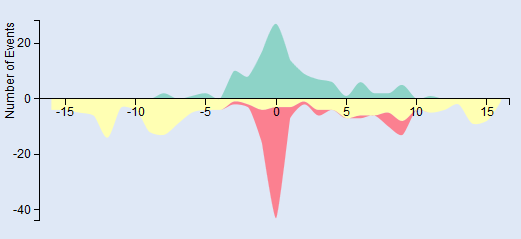
\includegraphics[width=0.4\textwidth]{stackedgraph_positive_neutral.png}%
\label{fig:positive-neutral}%
}

\caption{Different Layout of the Stacked Graph representing number of events over x-axis}
\end{figure}

For each stacked graph layout, user can choose which object type to show on the graph \ref{t13}. Options are available as radio button on top of the chart. Therefore, choosing Bonus will show only Positive and Neutral events, choosing Obstacle will show only Neutral and Negative events, and choosing Enemy will show all event type.

\subsection{Heat Map}
\begin{figure}
\centering
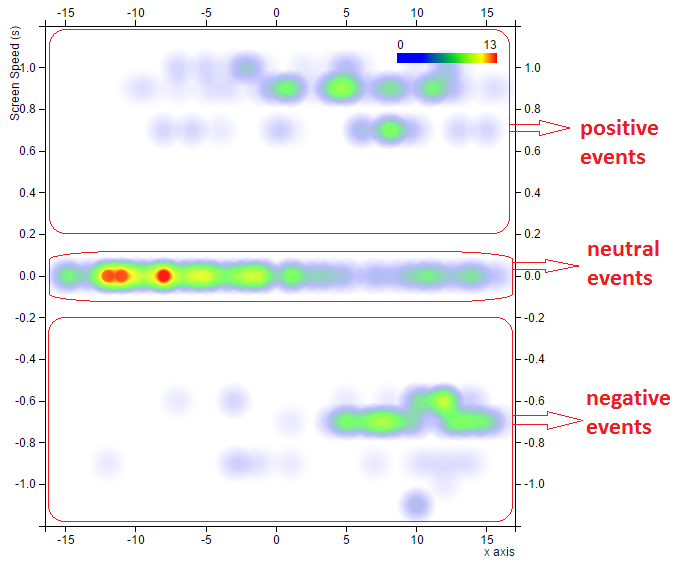
\includegraphics[width=130mm]{heatmap3.png}
\caption{Heatmap showing movement distribution over x-axis and screen speed}
\label{heatmap}
\end{figure}
Heat Map is a quite popular visualization method nowadays due to its ability which allows user to see variable with the highest value at one glance. Most of the time, heatmap is implemented on geographical map to represent variable value over certain area on map, i.e: Natural Disaster Risk by Location\footnote{\url{http://www.rms.com/}}, population density\footnote{\url{https://en.wikipedia.org/wiki/Population_density}}, Number of picture taken in an area\footnote{\url{http://sightsmap.com/}}, etc. Heat map is also used to track eye movement or mouse click on a website, and representing DNA microarray data in the form of cluster heat map\cite{friendly}. Heat map uses color gradation to represent the hotness level of a variable. Usually, red color is used to represent the high value (hot) and blue is used to represent the low value (cold). However, other color combination can also be used. To represent distribution of events and screen speed over x axis \ref{t12}, the events are first grouped based on their x values and normalized screen speed. The number of events is then represented as heat map on the graph with highest number of events in red color and the lowest number of events in blue color. Normalized screen speed is represented as vertical axis and x value is represented as horizontal axis. Using the same approach used in scatter plot chart, each event type is presented in different area: top for Positive, middle for Neutral, and bottom for Negative (Figure \ref{heatmap}). For Neutral events, the screen speed is not calculated since it basically mean an object has been avoided or missed. For Negative events, the screen speed is represented in negative to show that it's an uncalculated movement. For the heatmap, user can also choose to show a specific object \ref{t14} by clicking the radio button associated with the desired object.

\section{Summary Visualization}
The Summary Visualization fulfills the requirements concerning movement evolution over time (\textit{T}2.x). In this case, a single session is considered as a single time point. Since user are interested in evolution over a certain x-area, the visualization are divided into sections of x-area. There are three ways of division: by the range of x-area, by the number of events within an area, and by clustering. The following explains the three approaches and its interaction technique in details.

\subsection{Visualization by range of x-area}
To fulfill \ref{t21}, a streamgraph metaphor is chosen to show evolution of movement (represented by events) over time. 
Time is often displayed on x-axis, but here, x-axis represent the x-axis of the screen, so time is displayed on the y-axis. Some visualizations are also based on this approach, like Visual Sedimentation \cite{huron}. Here, sessions represent time with the earliest one shown at the bottom and the latest one shown on the top. The x axis is then divided into sections of the same range based on user input. For each section, events are then filtered to the one which happened within the section x boundary. The filtered events are grouped based on session number and event type. Number of events within this group is then presented in vertical streamgraph layout with event type represented using the same color used in the Session visualization (Figure  \ref{fig:type1_not_clustered}). 

Shown in Figure \ref{fig:type1_section} a section in the chart. Here, the lower x boundary is -20 and the upper x boundary is -7.33. Within this area, the evolution of events throughout all session can be seen\ref{t21}. It is also possible to see which session has the most or least number of events by comparing the total length of all event type in one session. 

\begin{figure}
\centering
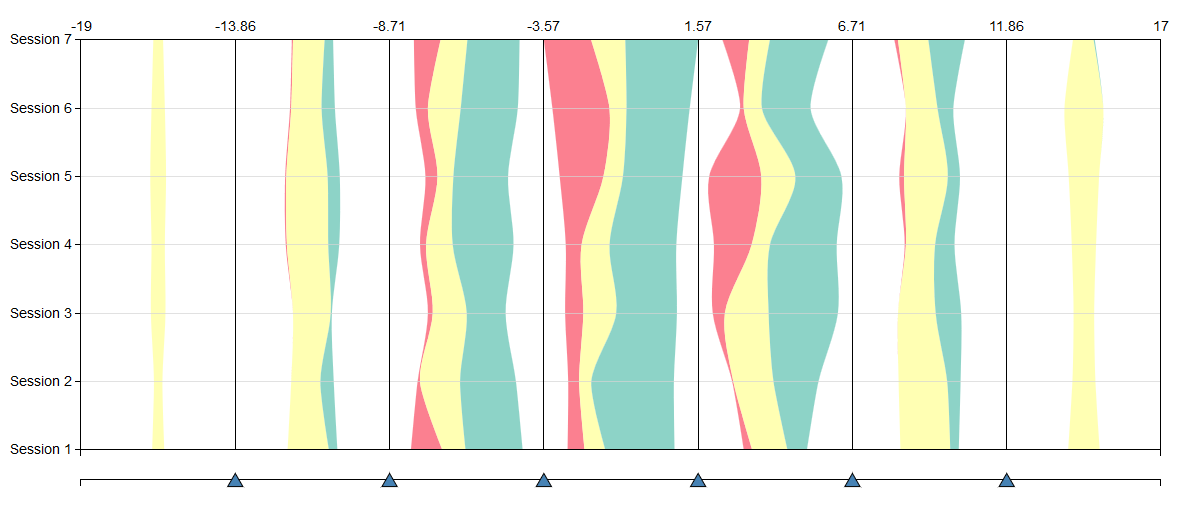
\includegraphics[width=130mm]{summary_not_clustered.png}
\caption{Summary Visualization divided by range of x-area}
\label{fig:type1_not_clustered}
\end{figure}

\begin{figure}
\centering
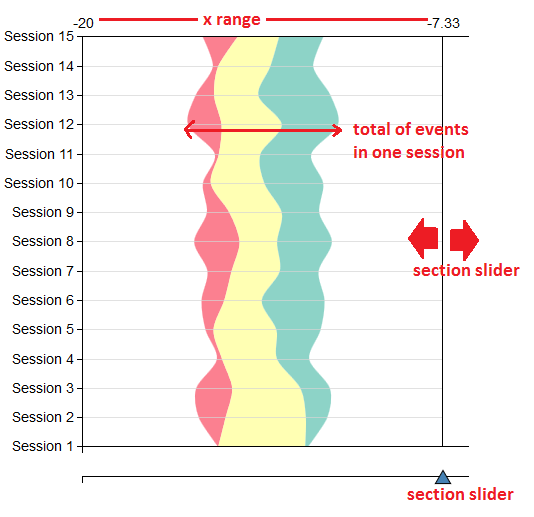
\includegraphics[width=80mm]{section.png}
\caption{A section in Summary Visualization}
\label{fig:type1_section}
\end{figure}

\begin{figure}
\centering
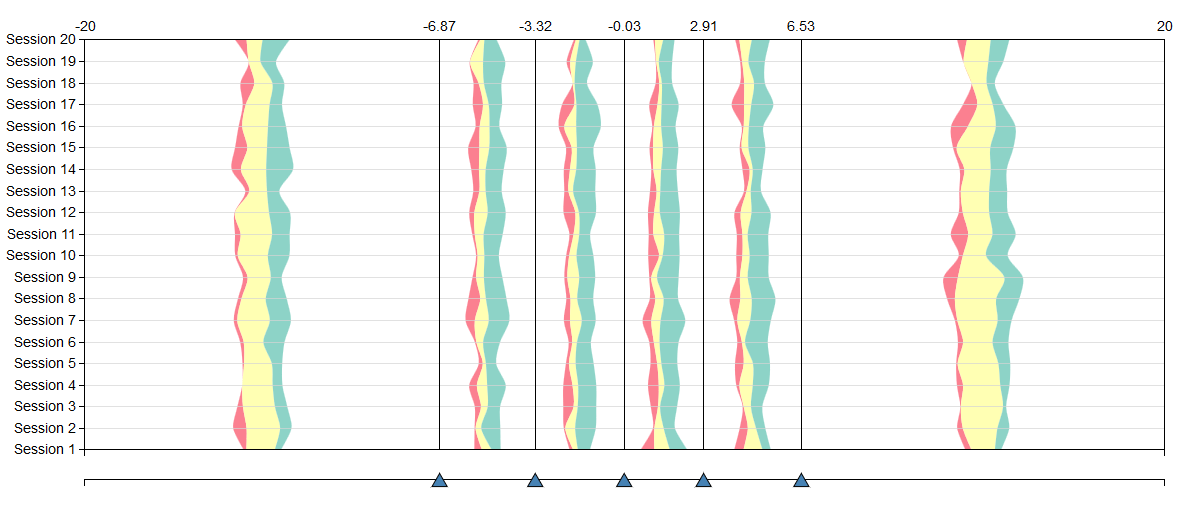
\includegraphics[width=130mm]{summary_type2.png}
\caption{Summary Visualization divided by number of events}
\label{fig:type2}
\end{figure}

\subsection{Visualization by number of events}
This second type of Summary Visualization uses the same approach explained previously. However, a section is calculated based on the total number of positive and negative events instead of the range of x-axis \ref{t23}. Therefore, based on the distribution of positive and negative events, one section in the chart may have bigger x-range than the other section. Only by comparing the size of sections, it's possible to know in which area most of the events are concentrated. Figure \ref{fig:type2} shows that the events are more concentrated in the middle area of the screen. Here, it can be concluded that on the far right and far left of the screen, there are more neutral events compare to the middle area.

\subsection{Visualization by clustering}
This third type of visualization fulfills \ref{t25}. As explained in section 4.2, initially the chart is divided into sections with range equals to an x-axis unit. Depending on the threshold value inputted by user, consecutive sections with distance below the threshold will be merged. This process is repeated until there is no sections with distance below the threshold. The input threshold ranges from 0 to 1. Thus, when user inputted threshold = 0, none of the section will be merged. On the other hand, when user inputted threshold = 1, all of the sections will be merged. Figure \ref{fig:type3_not_clustered} shows when user input threshold = 0, while Figure \ref{fig:type3_clustered} shows threshold = 0.24. As we can see, there are some sections which are merged, indicated with bigger section size. 4 sections are merged together forming one section with x range between 16-20 and 12-16. On the left side of the chart, 7 sections are merged together forming one big section ranging from -13 to -20.

\begin{figure}
\centering
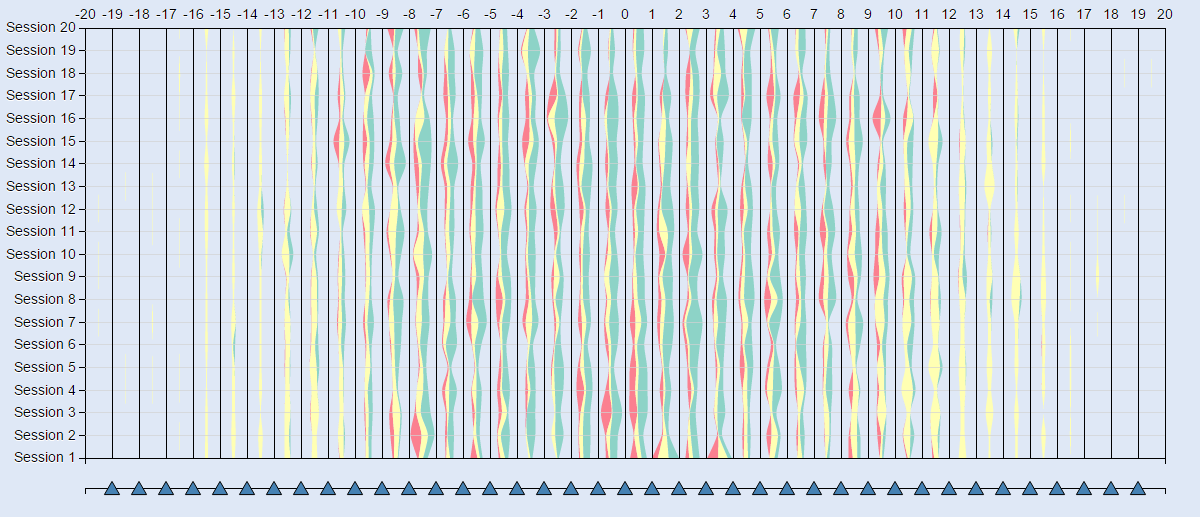
\includegraphics[width=150mm]{type3_not_clustered.png}
\caption{Summary Visualization divided by movement evolution similarity, clustered with threshold = 0}
\label{fig:type3_not_clustered}
\end{figure}

\begin{figure}
\centering
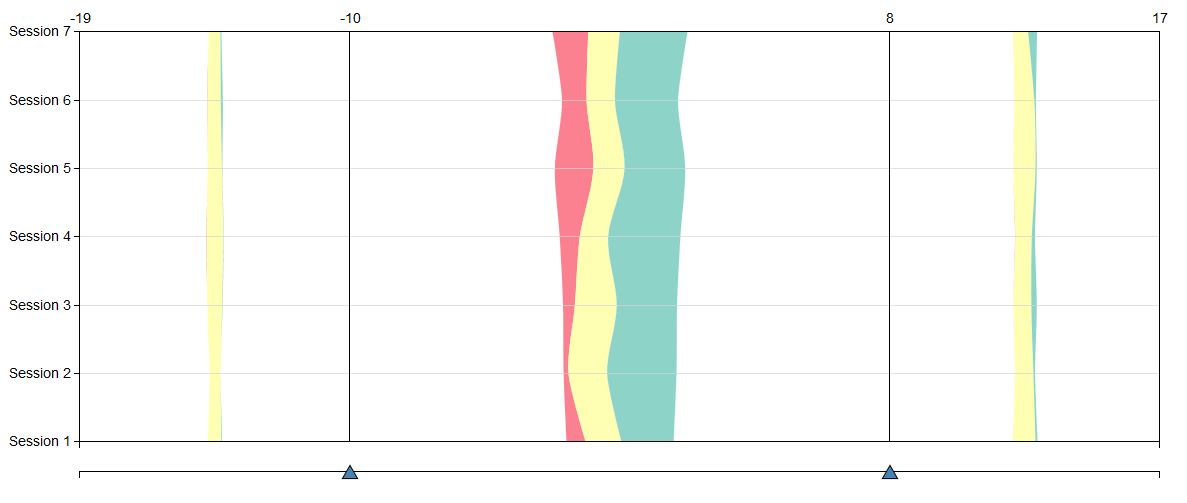
\includegraphics[width=150mm]{summary_clustered.png}
\caption{Summary Visualization divided by movement evolution similarity, clustered with threshold = 0.24}
\label{fig:type3_clustered}
\end{figure}

\subsection{Interaction Technique}
On top of the chart, an interaction bar is provided where user can interact with and change some variable in the chart. In first panel of the interaction bar (Figure \ref{fig:interaction_bar}), three sliders are provided: (i) slider to input the number of slices so that each section will have the same x-range (ii) slider to input the number of slices so that each section will have the same total number of positive and negative events (iii) slider to input threshold so that each section will have a cluster of similar movement evolution. When user uses slider (i) and (ii), the value on the slider defines the number of sections on the chart. For (i), the more number of sections, the smaller the x-range. While for (ii), the value selected on the slider is a denominator. The input is calculated by dividing total number of all positive and negative events by the value selected on the slider. Thus, the smaller the number chosen on the slider, the bigger the number of events. In the second panel, user has the options to choose which event type to show on the chart. This fulfills requirement \ref{t22} and \ref{t24}. By default all event type will be shown. 

Once the chart is generated, user has the ability to slide/drag the line between each session or the small triangle at the bottom of the line to the right or left(see Figure \ref{fig:type1_section}) to change the range of it's neighbouring sections\ref{t21}\ref{t23}. While dragging, the text on top of the line changes based on the current x value of the dragged line. When a line is dragged over another line, the two sections will be merged creating a new section with different x range. Therefore, user may be able to gain the information in which particular area a certain type of events starting to happened. Figure \ref{fig:line_dragging} shows changes on affected sections when line 11.63 is dragged to the left to position 10.7. We can see that Negative events on the circled area started to appears from x = 10.7. It is also possible to divide a section into two sections by clicking the top area of the chart in between the lower and upper section boundary text. This allows user to know the distribution of event type within a section.

\begin{figure}
\centering
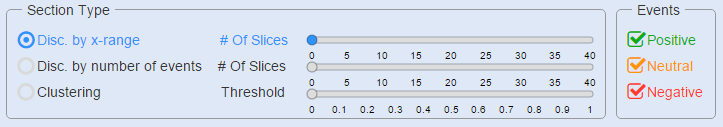
\includegraphics[width=130mm]{interaction_bar.png}
\caption{Interaction Bar for Summary Visualization}
\label{fig:interaction_bar}
\end{figure}
\begin{figure}
\centering
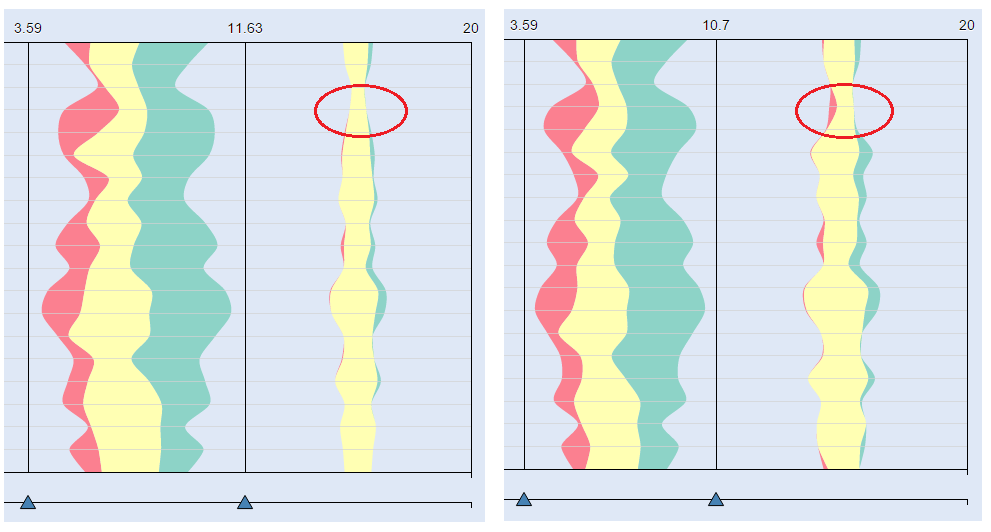
\includegraphics[width=110mm]{line_dragging.png}
\caption{Navigating section line to highlight pattern}
\label{fig:line_dragging}
\end{figure}

\section{General Interface}
\begin{figure}[H]
\centering
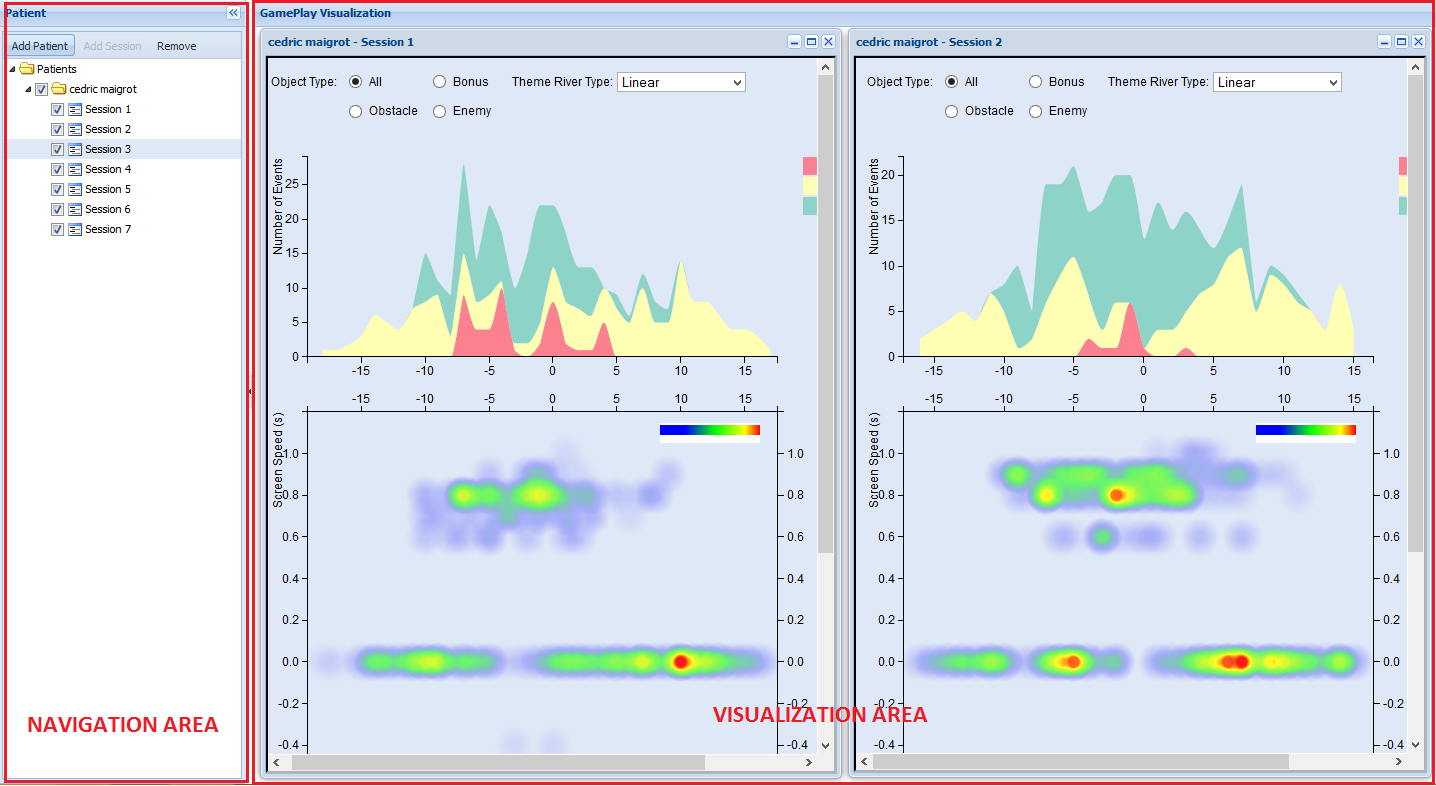
\includegraphics[width=150mm]{interface_app_compare.png}
\caption{Application Interface}
\label{fig:app_interface}
\end{figure}
Both the Session and Summary visualization are attached into an application which allows user to navigate different player and session. Unlike the visualization interface, the general interface is built using extjs library which allows the development of desktop-like web application. The interface of this application is divided into two areas: Navigation area and Visualization area (Figure \ref{fig:app_interface}). In Navigation area, user can choose patient and the sessions they have played. On clicking a session, a Session visualization of this session will be shown on the visualization area. It is also possible to open more than one Session visualization and rearrange the visualization window to compare gameplay between sessions (similar to navigating multiple windows in desktop). On clicking patient's name, Summary visualization for the chosen session will be shown.

\chapter{Case Studies}
write a kind of stories. Looking at this visualization, I see this and that. This correspond to this task and this task.
\section{Normal Player}
\section{Patient}
\chapter{Conclusion}

In this thesis we presented a visualization interface to help healthcare professionals analyse gameplay of Hammer and Planks, a serious game which is used to rehabilitate patient with balance disorder. Player movement, represented by events happened in the game world, are visualized in two type of views: (i) \textit{Session Visualization} which allows user to analyse movement in one session. (ii) \textit{Summary Visualization} which allows user to analyse movement evolution over several sessions. In both visualizations, events are categorized into Positive, Neutral, and Negative to help user intuitively understand player movement throughout the session. In (i) streamgraph paradigm is used to show player movement over x-axis which in turn provides the information to which direction (left or right) the player moves more. A more detailed view is provided with heatmap showing the pace of the game when each event happened. In (ii), x-axis is divided into sections and each section represents movement evolution throughout all sessions, shown in streamgprah. Here, three types of section division are provided to help user identify interesting movement pattern: by x-range, by number of events, and by clustering. In clustering view, we proposed a clustering method based on hierarchical clustering to aggregate similar movement patterns over consecutive sections. A distance formula which consider events proportion and evolution is presented to quantify the difference of movement pattern between section.

To evaluate the interface functionality, two case studies were discussed: one from healthy person and one from patient. Both discussed cases are able to show the effectiveness of the interface in achieving the tasks defined and therefore help the healthcare professionals assessing the progress of rehabilitation.

We identified some limitations in our research that could be improved in future work. First, the distance function used in the clustering algorithm is based on euclidean distance. Although currently this distance function are able to quantify the difference in events proportion and evolution, it will be interesting to investigate other distance function and to see if it can improve the clustering. Another limitation is the data set used in the case studies isn't accompanied with pathology information. It will be interesting to study different type of pathology and it's movement pattern. In the future, these data can be used to improve the game by proposing game setting based on the type and severity of pathology. Lastly, current interface only explore log data related to events. Log data related to skeleton movement of the players throughout the game hasn't been explore. For future work, an interface visualizing the body movement and identifying different kind of movement quality and quantity (repetition, smoothness, accuracy, etc.) can help healthcare professional to improve the quality of rehabilitation process.



%----------------------------------------------------------------------------------------
%	APPENDICES
%----------------------------------------------------------------------------------------

%\appendix%

%\chapter{Appendix Case Studies}
\label{chap:appendix1}




%

%----------------------------------------------------------------------------------------
%	BIBLIOGRAPHY
%----------------------------------------------------------------------------------------

\bibliography{Thesis}
\bibliographystyle{plain}


%\printnomenclature

%\cleardoublepage


\end{document}
